%%%%%%%%%%%%%%%%%%%%%%%%%%%%%%%%%%%
%%%%%%%%%%%%%%%%%bardproj_template.tex%%%%%%
%%
%% This is a template for the Bard Project Style.
%%
%% Copy it to a new file with a new name and use it as the basis
%% for your Bard senior project or M.A.T. mathematics research project.
%%
%% Replace everything inside <   > with the appropriate text,
%% and remove the <   >.
%%
%% Put a comment symbol (%) before anything in the template you 
%% do not need.
%%
%% Add as many additional chapters, sections and bibliographic 
%% entries as you need.
%%
%% Read the manual bardproj_man.tex or bardproj_man.pdf 
%% for more details regarding the Bard Project Style.
%%
%% The Bard Project Style file and the manual for this style file
%% can be found at http://math.bard.edu/bloch/bardtex.htm
%%
%% For additional help, or for suggestions or corrections
%% contact Ethan Bloch at bloch@bard.edu
%%
%%%%%%%%%%%%Bard Senior Project Style %%%%%%%%%
%%%%%%%%%%%%%%%%%%%%%%%%%%%%%%%%%%%

\documentclass[11pt, oneside, reqno]{book}
\usepackage{amssymb, amsthm, amsmath, amsfonts}
\usepackage{bardproj}
\usepackage{graphicx} %this used to be graphics, which maybe is wrong
%\usepackage{amsrefs}

% Packages added by me:
\usepackage{color}
\usepackage{caption}
\usepackage{subcaption}
\usepackage{bm}
\usepackage{url}
\usepackage[lite]{amsrefs}
\usepackage{enumitem}
\usepackage{float}
\setlist[enumerate]{itemsep=0mm}
% code adapted from http://tex.stackexchange.com/a/11483/3954
\usepackage{tikz}
\usetikzlibrary{shadows,calc}

% some parameters for customization
\def\shadowshift{4pt,-4pt}
\def\shadowradius{6pt}

\colorlet{innercolor}{black!60}
\colorlet{outercolor}{gray!05}

% this draws a shadow under a rectangle node
\newcommand\drawshadow[1]{
	\begin{pgfonlayer}{shadow}
		\shade[outercolor,inner color=innercolor,outer color=outercolor] ($(#1.south west)+(\shadowshift)+(\shadowradius/2,\shadowradius/2)$) circle (\shadowradius);
		\shade[outercolor,inner color=innercolor,outer color=outercolor] ($(#1.north west)+(\shadowshift)+(\shadowradius/2,-\shadowradius/2)$) circle (\shadowradius);
		\shade[outercolor,inner color=innercolor,outer color=outercolor] ($(#1.south east)+(\shadowshift)+(-\shadowradius/2,\shadowradius/2)$) circle (\shadowradius);
		\shade[outercolor,inner color=innercolor,outer color=outercolor] ($(#1.north east)+(\shadowshift)+(-\shadowradius/2,-\shadowradius/2)$) circle (\shadowradius);
		\shade[top color=innercolor,bottom color=outercolor] ($(#1.south west)+(\shadowshift)+(\shadowradius/2,-\shadowradius/2)$) rectangle ($(#1.south east)+(\shadowshift)+(-\shadowradius/2,\shadowradius/2)$);
		\shade[left color=innercolor,right color=outercolor] ($(#1.south east)+(\shadowshift)+(-\shadowradius/2,\shadowradius/2)$) rectangle ($(#1.north east)+(\shadowshift)+(\shadowradius/2,-\shadowradius/2)$);
		\shade[bottom color=innercolor,top color=outercolor] ($(#1.north west)+(\shadowshift)+(\shadowradius/2,-\shadowradius/2)$) rectangle ($(#1.north east)+(\shadowshift)+(-\shadowradius/2,\shadowradius/2)$);
		\shade[outercolor,right color=innercolor,left color=outercolor] ($(#1.south west)+(\shadowshift)+(-\shadowradius/2,\shadowradius/2)$) rectangle ($(#1.north west)+(\shadowshift)+(\shadowradius/2,-\shadowradius/2)$);
		\filldraw ($(#1.south west)+(\shadowshift)+(\shadowradius/2,\shadowradius/2)$) rectangle ($(#1.north east)+(\shadowshift)-(\shadowradius/2,\shadowradius/2)$);
	\end{pgfonlayer}
}

% create a shadow layer, so that we don't need to worry about overdrawing other things
\pgfdeclarelayer{shadow} 
\pgfsetlayers{shadow,main}

\newsavebox\mybox
\newlength\mylen

\newcommand\shadowimage[2][]{%
	\setbox0=\hbox{\includegraphics[#1]{#2}}
	\setlength\mylen{\wd0}
	\ifnum\mylen<\ht0
	\setlength\mylen{\ht0}
	\fi
	\divide \mylen by 120
	\def\shadowshift{\mylen,-\mylen}
	\def\shadowradius{\the\dimexpr\mylen+\mylen+\mylen\relax}
	\begin{tikzpicture}
	\node[anchor=south west,inner sep=0] (image) at (0,0) {\includegraphics[#1]{#2}};
	\drawshadow{image}
	\end{tikzpicture}
}

\newcommand{\Mod}[1]{\ (\text{mod}\ #1)}

\BibSpec{webpage}{%
	+{} {\PrintAuthors} {author}
	+{,} { \emph} {title}
	+{:} { \emph} {subtitle}
	+{}{ \parenthesize} {date}
	+{,} { \url} {url}
	%+{.} { Accessed \PrintDateField} {accessdate}
	+{.} { } {note}
	+{.} {} {transition}
}

%\usepackage{caption}
%\usepackage{setspace}

%<Your macros, if you have any>



\begin{document}

%For senior projects:
\titlepg{Development and Optimization of a Two-View Model for Anamorphic Projections on Planar Surfaces}{Van Mai Nguyen Thi}
    {May}{2015}

%For M.A.T. mathematics research projects, uncomment the following, and remove the above:
%\titlepgmat{<Title of Project>}{<Your Name>}
%    {<Month of Graduation>}{<Year of Graduation>}

\abstr

An anamorphic projection is an image that is intentionally distorted so that the original image can be seen only when looked at from a certain perspective, or using a special device, for example a mirror. Origins of anamorphosis can be traced back to the 16th century art, but beyond the aesthetic values, anamorphosis has found its uses in many practical settings, such as road signs, and keystone correction. Despite the widespread uses, there is a scarcity of detailed explanation of the mathematical principles behind anamorphosis, and there is hardly any computer software generating the anamorphic projections. The goal of this project is to apply computer vision techniques to create a program that automates the process of generating anamorphic projections. We use a projector-camera system to derive homography mappings between the projector and camera image, and propose a method for generating an optimal anamorphic image for multiple viewers using least squares. 

\tableofcontents

\listoffigures

\dedic

\begin{center}
\Large I dedicate this work to my family.
\end{center}


\acknowl

First of all, I would like to thank my advisors, Keith and Jim, for their constant advice, support and encouragement throughout this project.
In would like to thank Keith for his enthusiasm and support, from brainstorming ideas to finalizing this project. Thank you Jim for your guidance and contribution.
My thanks also go to the Mathematics and Computer Science departments for giving me the foundation to work on this project. 

I also want to thank my friends, Thinh, Linh, Jin, for supporting me with my project and the good memories that we have had at Bard. I also thank Georgia, Alexzandra and Eva-Marie for being great suitemates and helping me whenever I needed. 

I want to thank Thant Ko Ko for his continuous support and always being there for me.

Finally, I would like to thank my parents for their unconditional love and support throughout my life, and my little sister Ola for never failing to make me laugh.


\doublespace






%TODO CH1: Introduction Chapter (bg, definitions)
\chapter{Introduction}
\label{chap:int}

%%%%%%%%%%%%%%%%%%%%%%%%%%%%%%%%%%%%%%%%%%%%%
%%%   S E C T I O N   %%%%%%%%%%%%%%%%%%%%%%%%%%%%%%%%%
%%%%%%%%%%%%%%%%%%%%%%%%%%%%%%%%%%%%%%%%%%%%%

\section{Background}
\label{sec:bac}

An anamorphosis (or anamorphic projection/image) is an image that is intentionally distorted so that the original image can be recovered only when looked at from a certain point of view or using a special device, for example a mirror. Origins of anamorphosis can be traced back to the 16th century when artists, mathematicians and philosophers, fascinated by the idea of perspective, experimented with the notions of illusion, truth and reality~\cite{hunt2000anamorphic}. Some of the notable examples of anamorphosis include Jean-Francois Niceron's methods for geometrical construction that generated multiple types of anamorphic transforms which involved both exact and approximate methods~\cites{hunt2000anamorphic,niceron1992perspective}. One of the most famous anamorphic paintings is Hans Holbein's \textit{The Ambassadors} (Figure \ref{fig:hol}), in which the artist embedded an anamorphic image of a skull (Figure \ref{fig:hol_sku}) at the bottom of the painting as a \textit{memento mori}, a recurring motif in many artworks in the Renaissance period.

%\begin{figure}
%\centering
%\begin{minipage}{.46\textwidth}
%	\centering
%	\shadowimage[width=\linewidth]{data/Holbein1}
%	\captionof{figure}{Hans Holbein's \textit{The Ambassadors}, 1533 <Add reference>}%TODO add
%	\label{fig:hol}
%\end{minipage}%
%\qquad\begin{minipage}{.45\textwidth}
%	\centering
% 	\shadowimage[width=.9\linewidth]{data/Holbein_Skull}
%  	\captionof{figure}{Undistorted skull from H. Holbein's \textit{The Ambassadors} <Add reference>}%TODO add reference
%  	\label{fig:hol_sku}
%\end{minipage}
%\end{figure}

\begin{figure}[h]
\centering
\shadowimage[width=0.5\textwidth]{data/examples/Holbein_wiki}
\caption{Hans Holbein's \textit{The Ambassadors}, 1533}
\label{fig:hol}
\end{figure}

\begin{figure}[H]
\centering
\shadowimage[width=0.35\textwidth]{data/examples/Holbein_Skull_wiki}
\caption{Undistorted skull from H. Holbein's \textit{The Ambassadors}}
\label{fig:hol_sku}
\end{figure}

Anamorphosis is still prevalent to this day, and is incorporated in many new forms of art, most notably street art. The undying fascination for anamorphosis is manifested in numerous artworks centered around the anamorphic principle and using it to create a unique piece of art.
Beyond the aesthetic values, anamorphosis has found its uses in many practical settings, such as road signs that are elongated so that drivers' looking at them from a small angle above the ground can see the signs correctly (Figure \ref{fig:bik}), or inverted ``ambulance" signs that are designed to be reflected correctly in the rear-view mirrors. Principles similar to those of anamorphosis are also found in keystone correction, which is a method for eliminating some distortions of projection that may result from misaligning the projector with the projection screen.

Despite the widespread uses, there is a scarcity of detailed explanation of the mathematical principles behind anamorphosis in the context of computer vision, and even with the advanced technology there is hardly any computer software generating the anamorphic projections. 
The goal of this project is two-fold. First of all, we explore the mathematical principles behind the most common types of anamorphosis. Next, we combine these theories with computer vision techniques to create a program that automates the process of generating anamorphic projections.

\begin{figure}[h]
\centering
\includegraphics[width=0.5\textwidth]{data/examples/bikes}
\caption{Road sign in the shape of an elongated bike. Left: view from the top; right: view from a driver's perspective~\cite{hunt2000anamorphic}.}
\label{fig:bik}
\end{figure}














%%%%%%%%%%%%%%%%%%%%%%%%%%%%%%%%%%%%%%%%%%%%%
%%%   S E C T I O N   %%%%%%%%%%%%%%%%%%%%%%%%%%%%%%%%%
%%%%%%%%%%%%%%%%%%%%%%%%%%%%%%%%%%%%%%%%%%%%%

\section{Previous Work}
\label{sec:prev}

We build our research on previous works on the topics related to anamorphosis. The mathematical transformations involved in various types of anamorphosis are explained in~\cite{hunt2000anamorphic}. In particular, it describes the transformation of points between planar surfaces in perspective anamorphosis, which is the main focus of this project. 
Because of the lack of resources about anamorphosis in computer vision, we review other related research projects that employ methods that are applicable to anamorphosis. There have been some development in the area of keystone correction, a topic which greatly overlaps with our project as it uses a similar projector-camera setup and planar image transformation detection methods~\cite{sukthankar2001smarter, brazzini2005computer}. Besides keystone correction, further innovations of~\cite{brazzini2005computer} and~\cite{sukthankar2001smarter} include an interactive user experience through a laser pointer. 
Related but outside of the scope of our project is dynamic anamorphosis, which adapts the generated images to the position of the viewer by tracking the viewer in real-time~\cite{solina2007dynamic, ravnik2013dynamic}.
We refer to~\cite{szeliski2010computer} and~\cite{hartley2003multiple} for comprehensive explanations of fundamental computer vision techniques and methods to analyze images, including feature detection and image transformation. \cite{hartley2003multiple} also provides a complete description of the geometric principles behind multiple view systems and techniques for reconstructing a three-dimensional scene using projector camera systems. 
%sources also
%We refer to two textbooks Two sources that were of ....
%<Szeliski + Multiple View>

%This project focuses on perspective planar anamorphosis













%keystone + laser
%\bib{brazzini2005computer}{article}{
%title={Computer vision for interactive skewed video projection},
%author={Brazzini, Alessandro and Colombo, Carlo},
%booktitle={Image Analysis and Processing--ICIAP 2005},
%pages={139--146},
%year={2005},
%publisher={Springer}
%}








%%%%%%%%%%%%%%%%%%%%%%%%%%%%%%%%%%%%%%%%%%%%%
%%%   S E C T I O N   %%%%%%%%%%%%%%%%%%%%%%%%%%%%%%%%%
%%%%%%%%%%%%%%%%%%%%%%%%%%%%%%%%%%%%%%%%%%%%%

\section{Motivation}
\label{sec:motivation}

While the inspiration for this project originates from the intriguing use of anamorphosis in art, the motivation for our research is the scarcity of previous work exploring the broad applications of anamorphosis in computer vision. Through this project, we hope to contribute to and bring the attention to this overlooked subject. 

Most research on the related topics deals with reconstructing the three-dimensional geometry of a scene, for example using a Kinect device or a multiple camera system. This project, however, takes a different approach in that it not only uses the cameras to reconstruct the information about the scene, but also optimizes the projections for the camera views. This work focuses on developing anamorphic models for single and two view geometries, both of which have potential applications in visual and performance arts and can be used to enhance the viewers' experience and create unique and engaging visual effects. We employ anamorphic principles to optimize projected images for a multiple view model, which has further use in developing anamorphic imaging systems for a large theatrical audience. Another advantage to this simple projector-camera model is its relatively low cost, which means that it can be effectively incorporated into class curricula to facilitate computer vision learning. 

%Multiple-viewer model - application for performance arts to utilize anamorphic projections in their performances, and optimize it for a large audience.








%%%%%%%%%%%%%%%%%%%%%%%%%%%%%%%%%%%%%%%%%%%%%
%%%   S E C T I O N   %%%%%%%%%%%%%%%%%%%%%%%%%%%%%%%%%
%%%%%%%%%%%%%%%%%%%%%%%%%%%%%%%%%%%%%%%%%%%%%

\section{Summary of Results}
\label{sec:summary}

The results of this project are described in detail in Chapter~\ref{ch:results}. The findings in this work are built upon a review of the mathematical concepts pertinent to perspective anamorphosis and computer vision techniques, which are employed later in this project.

Chapter \ref{chap:math} discusses the mathematical principles of the Pinhole Camera Model and two-dimensional image transformations, and introduces the concept of homogeneous coordinates. The theoretical background explained in Chapter~\ref{chap:math} serves as a basis for computer vision applications and methods described in Chapter~\ref{chap:algorithmic}. Based on what we learn from the review of these concepts, we build three models for generating anamorphic projections on planar surfaces, discussed in Chapter~\ref{ch:results}. We first implement a basic planar model using a simple projector-camera system. We estimate the homography relations between the images in the system and generate anamorphic images for the camera view. Based on our observations of some limitations in this simple model, we develop an improved model which addresses some of these limitations. These two models are presented in Sections~\ref{sec:basicModel} and~\ref{sec:improveModel}, and a homography estimation method using linear least squares for single view models is explained in Subsection~\ref{ssec:leastSqHomograph}. Finally, Section~\ref{sec:2view} studies a two view model and Subsection~\ref{ssec:hEstimateHomogeneousLS} develops a new method of homography estimation using homogeneous least squares which we implement in Python as part of the algorithm for the two view model.

%Finally, we study a two view model and develop a new method for optimizing the projected image for two camera views, discussed in Section \ref{sec:2view}, and the me



















%%%%%%%%%%%%%%%%%%%%%%%%%%%%%%%%%%%%%%%%%%%%%%%%%%%%%%%
%%%   C H A P T E R   %%%%%%%%%%%%%%%%%%%%%%%%%%%%%%%%%
%%%%%%%%%%%%%%%%%%%%%%%%%%%%%%%%%%%%%%%%%%%%%%%%%%%%%%%
\chapter{Mathematical Concepts}
\label{chap:math}

This chapter defines some basic concepts and terminology needed to describe anamorphic projections. In particular, we present the pinhole camera model and introduce homogeneous representations of geometrical objects used in computer vision to facilitate performing image transformations.
%the least squares minimization method, which is an important optimization tool used throughout this project.


%\section{Basic Concepts}
%\label{sec:basicConcepts}
%In mathematics, geometric elements in a coordinate system are most commonly represented in Cartesian coordinates. 
%
%
%\begin{definition}[Taylor expansion]
%\label{def:taylorExpan}
%%TODO
%\end{definition}

%\begin{definition}
%\label{def:pixelImage}
%define a computer pixel image
%\end{definition}





%%%%%%%%%%%%%%%%%%%%%%%%%%%%%%%%%%%%%%%%%%%%%
%%%   S E C T I O N   %%%%%%%%%%%%%%%%%%%%%%%%%%%%%%%%%
%%%%%%%%%%%%%%%%%%%%%%%%%%%%%%%%%%%%%%%%%%%%%

\section{Pinhole Camera Model}

The pinhole camera model is one of the simplest camera models. Its principles were known in as early as the thirteenth century, and used in ``camera obscura."~\cite{burger2009digital}

The pinhole camera can be visualized as a closed box with a small hole on one side, and an image plane on the opposite side. The light rays, which are reflected from objects in the real world, enter the box through the pinhole, and land on the image plane, forming a $180^{\circ}$ rotated two-dimensional reflection, as shown in Figure \ref{fig:pinhole}. The same mechanism describes the process of human vision, in which the light passes the through the pupil of the eye.

\begin{figure}[t]
	\centering
	\includegraphics[width=0.6\textwidth]{data/pinhole_camera/pinhole_big}
	\caption{Graphical representation of the pinhole camera model.~\cite{burger2009digital}}
	\label{fig:pinhole}
\end{figure}



\subsection{Mathematical Description}

For a more rigorous explanation of the model, we introduce a three-dimensional coordinate system where $Z$ is the axis orthogonal to the pinhole and image plane, $X$ is the horizontal axis, and $Y$ is the vertical axis, and the origin is placed at the pinhole, as shown in Figure \ref{fig:pinhole}. The position of any point in the real world in front of the pinhole box can be represented with the $X, Y$ and $Z$ coordinates. The image plane has its own two-dimensional coordinate system with $x$ and $y$ axes parallel to the $X$ and $Y$ axes respectively, and the origin on the $Z\text{-axis}$ at a distance $f$ (focal length) from the pinhole. 

Using this model, we can easily predict where a point lands on the image plane given its three-dimensional position in the real world. Observe that the ray connecting the point in the real world and its reflection in the image plane forms two similar triangles on either side of the pinhole by projecting itself onto the $XZ\text{-plane}$. Given this observation, we define the position $(x,y)$ of a point on the image plane corresponding to the point $(X,Y,Z)$ in the real world as
\[
y = -f\frac{Y}{Z}, \text{ and } x = -f\frac{X}{Z}.
\]








%%%%%%%%%%%%%%%%%%%%%%%%%%%%%%%%%%%%%%%%%%%%%
%%%   S E C T I O N   %%%%%%%%%%%%%%%%%%%%%%%%%%%%%%%%%
%%%%%%%%%%%%%%%%%%%%%%%%%%%%%%%%%%%%%%%%%%%%%

\section{Homogeneous Representation}
\label{sec:homogeneousRepresent}
Homogeneous coordinates were first introduced by August Ferdinand M\"{o}bius, and later became a powerful tool with applications in computer vision and projective geometry~\cite{allardice1891barycentric, smith1896history}. The homogeneous system is an alternative to the standard Euclidean, or \textit{inhomogeneous} system as it solves some of its limitations. One limitation of the Euclidean system is that it allows only linear transformations that fix the origin to be represented as matrices. Another limitation is that it does not have a finite representation for a point or line at infinity. The homogeneous model solves this problem by introducing an extra dimension, which provides a convenient representation for points and lines at infinity, as described later in this section. Another benefit of using the homogeneous model, and the reason for its prevalence in computer vision, is that projective transformations can be represented as matrices, which offers a convenient way to perform such operations.

%TODO projective space: define or not define??
%\begin{definition}[Projective space]
%	
%\end{definition}



\begin{definition}
	\label{def:hpoint}
	Let $P$ be a finite point in $n$ dimensions, and $(x_1, x_2, ..., x_n)$ be its representation in Cartesian coordinates. A \textit{homogeneous representation of point} $P$ is any $(n+1)$-tuple $(\omega x_1, \omega x_2, ..., \omega x_n, \omega)$, where $\omega \not=0$. The last coordinate $\omega$ is called the homogeneous coordinate. A homogeneous representation of a finite point has a non-zero homogeneous coordinate, and a point at infinity has a zero homogeneous coordinate.
\end{definition}

The homogeneity of this representation lies in the fact that when a homogeneous point is multiplied by a scalar, it is still the same point and corresponds to the same Cartesian point.

A Cartesian point can be converted to a homogeneous representation by appending $\omega=1$ as the $(n+1)^{th}$ coordinate. A homogeneous point can be converted to a Cartesian point by dividing each of its coordinates by $\omega$, and removing the homogeneous coordinate.

\begin{example}
	\label{ex:cartHomo}
	Let $P_1$ be a two dimensional point with Cartesian coordinates $(x,y)$. A possible homogeneous representation of $P_1$ is $(x,y,1)$, or more generally $(x\omega, y\omega, \omega)$ for any $\omega \not= 0$. Let $P_2$ be another point in two dimensions with homogeneous representation $(x,y,\omega)$. $P_2$ can be represented in Cartesian coordinates as $\left(\frac{x}{\omega}, \frac{y}{\omega}\right)$.
\end{example}

\begin{definition}
\label{def:hline}
Let $l$ be a straight line in two dimensions defined by the equation $ax+by+c = 0$. Then $(a,b,c)$ is the \textit{homogeneous representation of line} $l$.
\end{definition}

The homogeneity is preserved in this line representation because $(\lambda a, \lambda b, \lambda c)$ represents the line $\lambda ax+ \lambda by+ \lambda c = 0$, which is the same as line $ax+by+c = 0$ represented by $(a, b, c)$, for any $\lambda \not=0$.

Additionally, it follows from the definition of a line that a point $P$ lies on a line $l$ if the dot product of the homogeneous representations of $P$ and $l$ are zero.

\begin{lemma}
\label{lem:intersect}
A point $P$ is the \textit{intersection of two-dimensional lines} $l_1$ and $l_2$ if and only if $P$ is the cross product of the homogeneous vector representations of $l_1$ and $l_2$.
\end{lemma}
\begin{proof} This proof consists of two parts. First, we show that the cross product of the homogeneous representations of two lines is the intersection point of those lines. Then we prove that an intersection of two lines must also be the cross product of the two lines.

Let $l_1$ and $l_2$ be two-dimensional non-parallel lines represented as $(a_1,b_1,c_1)$ and $(a_2,b_2,c_2)$ respectively. Their cross product is a point $P$ defined as
\begin{align}
	P = (a_1,b_1,c_1) \times (a_2,b_2,c_2) = (b_1c_2-b_2c_1, a_2c_1-a_1c_2, a_1 b_2 - a_2b_1). \label{lineIntersectionCross}
\end{align}
We verify that $P$ lies on both lines $l_1$ and $l_2$ by demonstrating that the dot product of $P$ with each line is zero. For line $l_1$ we obtain
\begin{align*}
 & a_1(b_1c_2-b_2c_1) + b_1(a_2c_1-a_1c_2) + c_1( a_1 b_2 - a_2b_1) \\
=\;& a_1b_1c_2 - a_1b_2c_1 + a_2b_1c_1-a_1b_1c_2 + a_1b_2c_1-a_2b_1c_1 \\
=\; & 0,
\end{align*}
which means that $P$ lies on $l_1$. Similarly, we obtain that $P$ lies on $l_2$:
\begin{align*}
& a_2(b_1c_2-b_2c_1) + b_2(a_2c_1-a_1c_2) + c_2( a_1 b_2 - a_2b_1) \\
=\;& a_2b_1c_2 - a_2b_2c_1 + a_2b_2c_1-a_1b_2c_2 + a_1b_2c_2-a_2b_1c_2 \\
=\;& 0.
\end{align*}
Since $P$ lies on both $l_1$ and $l_2$, $P$, which is the cross product of the two lines, is the intersection of those lines.

It remains to show that the intersection of two lines is also the cross product of the lines. Let $Q = \left(x, y, 1\right)$ be the intersection point of $l_1$ and $l_2$. Notice that without loss of generality, any homogeneous representation can be transformed to a form with the homogeneous coordinate being $1$. Because $Q$ is the intersection point, ot must lie on both lines, which means that the dot product of $Q$ with each line is zero. The dot product of $Q$ and $l_1$ is
\[
Q \cdot l_1 = (x,y,1) \cdot \left(a_1, b_1, c_1\right)
= a_1 x + b_1 y + c_1,
\]
and the dot product of $Q$ and $l_2$ is 
\[
Q \cdot l_2 = (x,y,1) \cdot \left(a_2, b_2, c_2\right)
= a_2 x + b_2 y + c_2.
\]
We need to solve the following system of equations for $x$ and $y$:
\begin{align*}
a_1 x + b_1 y + c_1 &= 0 \\
a_2 x + b_2 y + c_2 &= 0.
\end{align*}
We obtain the solution with a simple row reduction:
%TODO change so that matrix is [1,0][0,1]. Now it's reversed.
\begin{align*}
 & \left[
\begin{array}{ c c | c}
a_1 & b_1 & -c_1 \\
a_2 & b_2 & -c_2
\end{array}
\right] \\[2 pt]
	\sim 
& \left[
\begin{array}{ c c | c}
0 & a_2b_1 - a_1b_2 & a_1c_2-a_2c_1 \displaybreak\\
a_2 & b_2 & -c_2
\end{array}
\right] \\[2 pt]
	\sim 
& \left[
\begin{array}{ c c | c}
0 & 1 & \frac{a_1c_2-a_2c_1}{a_2b_1 - a_1b_2} \\ [6 pt]
a_2 & 0 & -c_2- \frac{a_1b_2c_2-a_2b_2c_1}{a_2b_1 - a_1b_2}
\end{array}
\right] \\[2 pt]
	\sim 
& \left[
\begin{array}{ c c | c}
0 & 1 & \frac{a_1c_2-a_2c_1}{a_2b_1 - a_1b_2} \\ [6 pt]
1 & 0 & \frac{b_2c_1 - b_1c_2}{a_2b_1 - a_1b_2}
\end{array}
\right].
\end{align*}
Therefore the coordinates of $Q$ are
\[
	\left( \frac{b_2c_1 - b_1c_2}{a_2b_1 - a_1b_2},\frac{a_1c_2-a_2c_1}{a_2b_1 - a_1b_2}, 1 \right),
\]
which in homogeneous representation is equivalent to $\left(b_2c_1 - b_1c_2, a_1c_2-a_2c_1, a_2b_1 - a_1b_2\right)$, which is the cross product of $l_1$ and $l_2$, as computed in the equation (\ref{lineIntersectionCross}). Thus, the intersection point of two lines is also the cross product of the two lines.
\end{proof}


\begin{definition}
	The \textit{degrees of freedom} of a system is the number of independent parameters that define the system and are free to vary.
\end{definition}

\begin{example}
	 It is clear that a Cartesian point in two dimensions is defined by two parameters: the $x$ and $y$ coordinate. Thus a 2D point has two degrees of freedom. It is less obvious that a line in two dimensions has two degrees of freedom. Recall that a line is defined by an equation of the form $ax + by = c$, where the coefficients $a, b$ and $c$ define the line. Although this equation has three coefficients, a line is unique only up to a scale of the coefficients, that is a line $ax + by = c$ is the same as a line $sax + sby = sc$ for any non-zero scalar $s$. In fact, a line can be defined with two independent parameters: the slope and the $y$-intercept, marked as $m$ and $c$ in this common notation: $y = mx + c$.
\end{example}



% END of Homogeneous representation section




%%%%%%%%%%%%%%%%%%%%%%%%%%%%%%%%%%%%%%%%%%%%%
%%%   S E C T I O N   %%%%%%%%%%%%%%%%%%%%%%%%%%%%%%%%%
%%%%%%%%%%%%%%%%%%%%%%%%%%%%%%%%%%%%%%%%%%%%%

\section{2D Transformations}
\label{sec:2DTransform}

This section deals with types graphical transformations on 2D images. In computer vision, these operations are functions of pixel coordinates that return new coordinates for the given pixel. The simplest types of transformations include translation, rotation and affine. They form a basis for the projective transformation (homography), which could be thought of as an advanced transformation that includes but is not limited to a combination of those basic transformations. The projective transformation is defined in this chapter and discussed in more detail in Section \ref{sec:projectiveTransform}. The procedure of applying a transformation to an image is referred to as warping. There are two main methods of warping, defined in Subsection \ref{ssec:warping}.

%%%%%%%%%%%%%%%%%%%%%%%%%%%%%%%%%%%%%%%%%%%%%
%%%   S U B S E C T I O N   %%%%%%%%%%%%%%%%%
%%%%%%%%%%%%%%%%%%%%%%%%%%%%%%%%%%%%%%%%%%%%%

\subsection{Transformations}
\label{ssec:transformations}

This section focuses on some fundamental transformations of two dimensional images, illustrated in Figure \ref{fig:2dTransformations}. For each transformation, we provide a definition and present a matrix notation that offers a convenient way to apply them to 2D images. Since the transformations discussed here do not preserve the origin, their matrix notation is only possible when we use homogeneous coordinates, introduced in Section \ref{sec:homogeneousRepresent}.

\begin{figure}[h]
	\centering
	\includegraphics[width=0.9\textwidth]{data/2Dtransformations}
	\caption{Examples of basic 2D transformations. \cite{szeliski2010computer}}
	\label{fig:2dTransformations}
\end{figure}

\begin{definition}%[Translation]  
	\label{def:translation}
	\textit{Translation} is a type of transformation that shifts an image by a vector. It is typically defined as a $2\times3$ matrix 
	\[
	T = \begin{pmatrix}
	1 & 0 & t_x \\
	0 & 1 & t_y
	\end{pmatrix}
	\]
	or as a $3\times3$ matrix
	\[ 
	T = \begin{pmatrix}
	1 & 0 & t_x \\
	0 & 1 & t_y \\
	0 & 0 & 1
	\end{pmatrix}.
	\]
	for some translation factors $t_x$ and $t_y$.
\end{definition}

The $2\times3$ matrix can be applied to a homogeneous point this way:
\[
\begin{pmatrix}
x' \\ y'
\end{pmatrix}
= 
\begin{pmatrix}
1 & 0 & t_x \\
0 & 1 & t_y
\end{pmatrix}
\begin{pmatrix}
x \\ y \\ 1
\end{pmatrix}
= 
\begin{pmatrix}
x + t_x \\
y + t_y
\end{pmatrix}
\]
where $\left(x, y, 1\right)$ is initial position, and $\left(x', y'\right)^T$ is the new position after translation. Observe that the result of translation using the $2\times 3$ matrix is a point in Euclidean coordinates, without the homogeneous coordinate. This creates a significant disadvantage as it prevents combining several transformations. For example, if we want to apply another translation on this result, we need to convert it to the homogeneous coordinates first.

The $ 3\times 3 $ matrix gives the same result, but in homogeneous coordinates:
\[ 
\begin{pmatrix}
x' \\ y' \\ 1
\end{pmatrix}
=
\begin{pmatrix}
1 & 0 & t_x \\
0 & 1 & t_y \\
0 & 0 & 1
\end{pmatrix}
\begin{pmatrix}
x \\ y \\ 1
\end{pmatrix}
= 
\begin{pmatrix}
x + t_x \\
y + t_y \\
1
\end{pmatrix}.
\]
This notation makes it easy to apply another transformation such as translation directly to the result, as the result is already in the homogeneous form.

\begin{definition}%[Rotation]  
	\label{def:rotation}
	\textit{Rotation} is a type of transformation that preserves orientation, lengths and angles. In the most compressed form it is defined as a $ 2\times 2 $ matrix $R$:
	\[ 
	R = \begin{pmatrix}
	\cos\theta & -\sin\theta \\
	\sin\theta & \cos\theta
	\end{pmatrix} 
	\]
	for some angle $\theta$. In this $2\times 2$ form, rotation is applied to an Euclidean point, and the result is also in Euclidean form, and is the position of the initial point rotated by the angle $\theta$ around the origin. Another more versatile form of the rotation matrix is
	\[
	R = \begin{pmatrix}
	\cos\theta & -\sin\theta & 0 \\
	\sin\theta & \cos\theta  & 0 \\
	0 & 0 & 1
	\end{pmatrix} ,
	\]
	which is applied to a homogeneous point, and returns a rotated homogeneous point.
\end{definition}


\begin{definition}%[Scaling]  
	\label{def:scaling}
	\textit{Scaling} is a transformation that preserves orientation and angles. It takes a form of a non-zero scaling factor $s$, which can be applied to both homogeneous and inhomogeneous points.
\end{definition}

Rather than appearing separately, translation, rotation and scaling are often combined to create more complex transformations. For example, a combination of rotation and translation is called \textit{rigid} or \textit{Euclidean} transformation, and is of the form
\[
\begin{pmatrix}
\cos\theta & -\sin\theta & t_x \\
\sin\theta & \cos\theta  & t_y
\end{pmatrix}.
\]
A combination of all three basic transformations (translation, rotation and scaling) is referred to as \textit{similarity transform} is defined as
\[
\begin{pmatrix}
s\cos\theta & -s\sin\theta & st_x \\
s\sin\theta & s\cos\theta  & st_y
\end{pmatrix}
\]
or more generally as
\[
\begin{pmatrix}
a & -b & t_x \\
b & a  & t_y
\end{pmatrix}.
\]

\begin{definition}%[Affine]  
	\label{def:affine}
	An \textit{affine} transformation is a type of transformation that preserves parallel lines. It takes the form of any $2 \times 3$ matrix
	\[
	\begin{pmatrix}
	a_{00} & a_{01} & a_{02} \\
	a_{10} & a_{11} & a_{12}
	\end{pmatrix}.
	\]
\end{definition}

%TODO semi-proof that any 2x3 matrix  is affine (preserves parallel lines)?
%{\color{red}semi-proof that any 2x3 matrix  is affine (preserves parallel lines)?}


%%%%%%%%%%%%%%%%%%%%%%%%%%%%%%%%%%%
%%%%%%% H O M O G R A P H Y %%%%%%%
%%%%%%%%%%%%%%%%%%%%%%%%%%%%%%%%%%%

\begin{definition}%[Homography]  
	\label{def:homography}
	A \textit{homography}, also known as \textit{projective transformation} or \textit{perspective transform} is a transformation of a two-dimensional image $I$ to another two-dimensional image $I'$ (referred to as the anamorphic image), such that all straight lines in $I$ are preserved in~$I'$. It is represented as a $3 \times 3$ matrix
	\[
	\begin{pmatrix}
	h_{00} & h_{01} & h_{02} \\
	h_{10} & h_{11} & h_{12} \\
	h_{20} & h_{21} & h_{22}
	\end{pmatrix}.
	\]
\end{definition} 

%\begin{theorem}
%	\label{thm:homographymatrix} 
%	A homography $H$ is an invertible $3 \times 3$ matrix. An anamorphic image is obtained by applying the homography $H$ to every point in the original image to obtain the corresponding points in the anamorphic image:
%	\[ p'=Hp \text{, for all points } x\in I. \] %TODO looks like same x', different x...
%	Line preservation means that the points $p_0, p_1, p_2 \in I$ lie on the same line if and only if $Hp_0, Hp_1, Hp_2$ are on the same line.
%\end{theorem}
%\begin{proof}
%	%TODO prove this 2 ways 
%	$\to$ show that any 3x3 matrix preserves lines \\
%	$\from$ derive the transformation on x and y is linear fractional for each coordinate. Then show that adding the third coordinate $\omega$ allows us to write the transformation as 3 linear transformations on $x,y,\omega$, written as a $3 \times 3$ matrix. \\
%	+ prove that $H$ is invertible
%\end{proof}

\begin{lemma} \label{lem:H=lambdaH}
	A homography $H$ produces the same transformation as a homography $\lambda H$ for any non-zero $\lambda$. 
\end{lemma}

\begin{proof}
	Let $p = \left(x, y\right)^T$ be a point in 2D, and $H$ be a homography matrix defined as:
	\[
	H = \begin{bmatrix} 
	h_{00} & h_{01} & h_{02} \\
	h_{10} & h_{11} & h_{12} \\
	h_{20} & h_{21} & h_{22}
	\end{bmatrix}.
	\]
	By Definition \ref{def:hpoint}, $\left(x, y, 1\right)^T$ is a homogeneous representation of $p$. Let  point $q$ be the result of the homography transformation $H$ on the homogeneous point $p$. Then 
	\[
	q = Hp = \begin{bmatrix}
	h_{00}x + h_{01}y + h_{02} \\
	h_{10}x + h_{11}y + h_{12} \\
	h_{20}x + h_{21}y + h_{22}
	\end{bmatrix}
	= \begin{bmatrix}
	\frac{h_{00}x + h_{01}y + h_{02}}{h_{20}x + h_{21}y + h_{22}} \\[6 pt]
	\frac{h_{10}x + h_{11}y + h_{12}}{h_{20}x + h_{21}y + h_{22}} \\[4 pt]
	1
	\end{bmatrix}.
	\]
	The last step of the derivation of $q$ is valid because a homogeneous point remains unchanged when multiplied by a scalar.
	
	Let $H'$ be another homography defined as $H' = \lambda H$ for some non-zero $\lambda$. Let $q' $ be the result of the homography $H'$ on $p$. Then 
	\[
	q' = H'p = \begin{bmatrix}
	\lambda\left(h_{00}x + h_{01}y + h_{02}\right) \\[3 pt]
	\lambda\left(h_{10}x + h_{11}y + h_{12}\right) \\[3 pt]
	\lambda\left(h_{20}x + h_{21}y + h_{22}\right)
	\end{bmatrix}
	= \begin{bmatrix}
	\frac{\lambda\left(h_{00}x + h_{01}y + h_{02}\right)}
	{\lambda\left(h_{20}x + h_{21}y + h_{22}\right)} \\[7 pt]
	\frac{\lambda\left(h_{10}x + h_{11}y + h_{12}\right)}
	{\lambda\left(h_{20}x + h_{21}y + h_{22}\right)} \\[5 pt]
	1
	\end{bmatrix}
	= \begin{bmatrix}
	\frac{h_{00}x + h_{01}y + h_{02}}{h_{20}x + h_{21}y + h_{22}} \\[7 pt]
	\frac{h_{10}x + h_{11}y + h_{12}}{h_{20}x + h_{21}y + h_{22}} \\[5 pt]
	1
	\end{bmatrix}.
	\]
	Thanks to the property of scalar invariance of the homogeneous representation, the two transformations $H$ and $H' = \lambda H$ are the same.
\end{proof}

By Lemma \ref{lem:H=lambdaH}, projective transformation matrices are invariant to scale, and therefore have eight degrees of freedom. This fact is of particular significance as we introduce a method for homography estimation that uses this property in Section~\ref{sec:projectiveTransform}. 











%%%%%%%%%%%%%%%%%%%%%%%%%%%%%%%%%%%%%%%%%%%%%
%%%   S E C T I O N   %%%%%%%%%%%%%%%%%%%%%%%%%%%%%%%%%
%%%%%%%%%%%%%%%%%%%%%%%%%%%%%%%%%%%%%%%%%%%%%

\subsection{Warping}
\label{ssec:warping}

Definitions \ref{def:translation} through \ref{def:homography} are different types of two-dimensional transformations. The process of applying a transformation, or a combination of transformations to an image is called warping. We distinguish two basic types of warping: forward and backward, which differ in that forward warping directly transforms the original image to the final image, while backward warping fills in each pixel of the final image with the corresponding color from the original image.

\begin{definition}[Forward Warping]  
	\label{def:forwarp}
	Let $t$ be a transformation function that maps pixels from image $I$ to another image $I'$. An image can be forward warped by copying the color at each pixel at point $p \in I$ to a point $p' \in I'$, where $p' = t(p)$.
\end{definition}

\begin{definition}[Backward Warping]  
	\label{def:backwarp}
	Let $t$ be a transformation function that maps pixels from image $I$ to another image $I'$, and $t^{-1}$ be the inverse warping that maps pixels from $I'$ to $I$. An image can be backward warped by iterating through points $p' \in I'$, and ``coloring" it with the color at the point $p \in I$, where $p = t^{-1}(p')$. 
	
\end{definition}

%TODO PSEUDOCODE for forward/backward warping
%{\color{red}PSEUDOCODE for forward/backward warping}

%TODO Warping: Diagrams
%{\color{red}Warping: Diagrams}
%TODO Pros & Cons of forward and backward
%{\color{red}Pros \& Cons of forward and backward}

In practice, warping is often improved by some methods of interpolation that take into account a cluster of pixels to determine the best color for each pixel on the final image, rather than copying a single pixel from the original image. Interpolation is designed to create smoother and more accurate color transitions, and further minimizes the distortions generated by warping. In this project, we use a warping method provided by the OpenCV library which uses bilinear interpolation and nearest-neighbor interpolation~\cite{opencvfeaturedetection}. 
%The linear interpolation determines the color value at each pixel by averaging over the pixels 
These interpolation methods determine the color value at each pixel by averaging over the pixels around it.

% END of 2D Transformations subsection




%%%%%%%%%%%%%%%%%%%%%%%%%%%%%%%%%%%%%%%%%%%%%
%%%   S E C T I O N   %%%%%%%%%%%%%%%%%%%%%%%%%%%%%%%%%
%%%%%%%%%%%%%%%%%%%%%%%%%%%%%%%%%%%%%%%%%%%%%

%TODO should this be here at all?
%\section{Anamorphosis}
%\label{sec:typesAnamorphosis}
%
%\begin{definition}[Perspective anamorphosis]
%\label{def:perspective}
%Let $S$ be a surface and $V$ be a viewer at some distance $d$ looking directly at the surface $S$ at some angle $\theta$. Let $I$ be some two-dimensional image. $I’$ is an anamorphic projection of $I$ on the surface $S$ for the viewer $V$ if the resulting image that $V$ sees when looking at $S'$ is $S$.
%\end{definition}
%
%\begin{definition}[Planar anamorphosis]
%\label{def:planar}
%This is my definition of planar anamorphosis. 
%\end{definition}

%\begin{definition}[Mirror anamorphosis]
%\label{def:mirror}
%This is my definition of mirror anamorphosis. 
%\end{definition}












%%%%%%%%%%%%%%%%%%%%%%%%%%%%%%%%%%%%%%%%%%%%%%%%%%%%%%%
%%%   C H A P T E R   %%%%%%%%%%%%%%%%%%%%%%%%%%%%%%%%%
%%%%%%%%%%%%%%%%%%%%%%%%%%%%%%%%%%%%%%%%%%%%%%%%%%%%%%%

%TODO CH3: Anamorph (Theory/Math) Chapter
\chapter{Algorithmic Methods}
\label{chap:algorithmic}

This chapter deals with the techniques and methods used in the implementation of the automated anamorphic projection program that we develop in this project. We introduce the linear least squares minimization method, which is a crucial tool for estimating the projective transformations of various surfaces in our anamorphic model, which we discuss in more detail in Chapter \ref{ch:results}. We also explain the main feature detection algorithms such as Harris Corner Detection and Chessboard Corner Detection, which are used to facilitate the process of computing the transformations.



%%%%%%%%%%%%%%%%%%%%%%%%%%%%%%%%%%%%%%%%%%%%%
%%%   S E C T I O N   %%%%%%%%%%%%%%%%%%%%%%%%%%%%%%%%%
%%%%%%%%%%%%%%%%%%%%%%%%%%%%%%%%%%%%%%%%%%%%%

\section{Least Squares Minimization Method}
\label{sec:leastSquares}

The least squares method is a technique to estimate the best possible solution to a system of equations, which is especially useful when the exact solution to that system does not exist. This approach is designed to solve overdetermined systems, which means that there are more equations than unknowns. This estimate is obtained by searching for a solution that minimizes the error, defined as the sum of squared differences of the result of the estimated solution and the desired result. One of the most prevalent uses of this method is in finding the line of best fit to a set of data points, such that the sum of the squared vertical distances from the line to each data point is minimized. 
The least squares model can be used to predict the outcomes of the points not included in the finite input data. For example, the line of best fit provides a prediction of the outcomes for all points in the domain, and not just the input data points.
Because of its application as an error minimization method, the least squares estimation is used in many optimization problems in practical experiments to minimize the errors resulting from inaccuracies of a practical setup. For the same reason, it is of great significance to this project as it is the main technique to estimate projective transformations between the computer screen image, camera image, and the projective screen. 

We distinguish two types of least squares methods: linear and non-linear least squares. The linear least squares is an approach for finding the model that best describes a set of input and output data, in which for pair of corresponding input and output data points, the model can be expressed as a linear function of the parameters. Notice that the linear least squares model is not necessarily a linear function in terms of the data points. For example $f(x) = ax^2 + b\log(x)$ is a valid model because $f(x_i) = ax_i^2 + b\log(x_i)$ is linear in terms of the coefficients $a$ and $b$ for all data points $x_i$. On the contrary, the non-linear model is not linear in terms of the coefficients, although some non-linear models can be transformed into linear models, for example the non-linear model $g(x) = e^{ax}$ can be transformed into $h(x) = \ln\left(g(x)\right) = ax$ with the output data being $\ln(y)$ instead of just $y$. We mentioned that the least squares solves overdetermined systems. This means that for an assumed model with $m$ coefficients $a_1, a_2, \dots a_m$ we need $n$ input data points, and $n$ corresponding output points, where $n \ge m$. 

This section deals with the linear least squares as it is the method used in this project. We demonstrate the method of finding the least squares solution on a simple linear model, and a more general model.
%explain the method for homography estimation using the least squares.
%\color{red}<Explain general least squares minimization. Appendix 5, p.>

%\subsection{Linear Least Squares on a Linear Model}

\subsection{Linear Model}
	This is an example of the linear least squares on a linear regression model.
	
	Let $f: \mathbb{R} \to \mathbb{R}$ be a linear function that models the data with input $\{x_1, x_2, \dots, x_n\}$ and observed output $\{y_1, y_2, \dots, y_n\}$, where $n \ge 2$. The function $f$ is of the form $f(x) = mx+c$ for some coefficients $m$ and $c$, where $m\not= 0$. In order for $f$ to be a ``good" model of the data, we need to pick the values of $m$ and $c$ so that $f(x_i) \approx y_i$ for all $1 \le i \le n$.
	
	We define an error function $E$ as $E(m,c) = \sum_{i=1}^n \left(f(x_i) - y_i\right)^2$. To shorten the derivations and make it easier to read, we assume that all summations $\sum_i$ in this subsection are equivalent to $\sum_{i=1}^n$. The error function serves as a measure of how well $f$ represents the data. We need to find $m$ and $c$ such that the value of $E(m, c)$ is closest to $0$. Because $E$ is always positive ($E$ is a sum of squares), this statement is equivalent to finding $m$ and $c$ at the minimum of $E$. In order to find the minimum of $E$, we take the partial derivative of $E$ with respect to each of its arguments, and solve the system of equations in which each derivative is equal to~$0$. 
	The partial derivative of $E$ with respect to $m$ is
	\begin{align*}
	\frac{\partial}{\partial m} E(m,c) 
	&= \frac{\partial}{\partial m} \sum_i \left(mx_i+c-y_i\right)^2 \\
	&= \sum_{i} 2x_i \left(mx_i + c - y_i\right) \\
	&= \left(\sum_{i} 2x_i^2\right) m 
	+ \left(\sum_{i} 2x_i \right) c
	- \left(\sum_{i} 2x_iy_i\right).
	\end{align*}
	The partial derivative of $E$ with respect to $c$ is
	\begin{align*}
	\frac{\partial}{\partial c} E(m,c) 
	&= \frac{\partial}{\partial c} \sum_{i} \left(mx_i+c-y_i\right)^2 \\
	&= \sum_{i} 2 \left(mx_i + c - y_i\right) \\
	&= \left(\sum_{i} 2x_i\right) m 
	+ (2n) c
	- \left(\sum_{i} 2y_i\right).
	\end{align*}
	We set each derivative to zero and solve the simple system of linear equations in which the first column contains the coefficients of $m$, and the second column corresponds to the coefficients of $c$, and the last column has the constant terms of the resulting equations:
	\[
	\left[
	\begin{array}{c c | c}
	\sum_{i} x_i^2 & \sum_{i} x_i & \sum_{i} x_iy_i \\ [7 pt]
	\sum_{i} x_i   & 	n 			  & \sum_{i} y_i 
	\end{array}
	\right].
	\]
	We perform a simple row reduction to transform it to the reduced row echelon form:
	\begin{align*}
	& \left[
	\begin{array}{c c | c}
	\sum_{i} x_i^2 & \sum_{i} x_i & \sum_{i} x_iy_i \\[8 pt]
	\sum_{i} x_i   & 	n 			  & \sum_{i} y_i 
	\end{array}
	\right] \\[8 pt]
		\sim & \left[
	\begin{array}{c c | c}
	n\left( \sum_{i} x_i^2 \right) - \left(\sum_{i} x_i\right)^2 
	& 0 
	& n\left(\sum_{i} x_iy_i\right) - \left(\sum_{i} x_i\right)\left(\sum_{i} y_i\right) \\[8 pt]
	\sum_{i} x_i & n & \sum_{i} y_i 
	\end{array}
	\right] \\[8 pt]
		\sim & \left[
	\begin{array}{c c | c}
	1 & 0 & \frac{ \left(n\sum_{i} x_iy_i\right) - \left(\sum_{i} x_i\right)\left(\sum_{i} y_i\right) }
	{ \left(n\sum_{i} x_i^2\right) - \left(\sum_{i} x_i\right)^2 } \\[13 pt]
	0 & n & \sum_{i} y_i - \frac{\left(n\sum_{i} x_iy_i\right)\left(\sum_{i} x_i\right) - \left(\sum_{i} x_i\right)^2 \left(\sum_{i} y_i\right)}
	{ \left(n\sum_{i} x_i^2\right) - \left(\sum_{i} x_i\right)^2}
	\end{array}
	\right] \\[8 pt]
		\sim & \left[
	\begin{array}{c c | c}
	1 & 0 & \frac{ \left(n\sum_{i} x_iy_i\right) - \left(\sum_{i} x_i\right)\left(\sum_{i} y_i\right) }{ \left(n\sum_{i} x_i^2\right) - \left(\sum_{i} x_i\right)^2 } \\[13 pt]
	0 & 1 & \frac{\sum_{i} y_i}{n} + \frac{\left(\sum_{i} x_i\right)^2 \left(\sum_{i} y_i\right) - \left(n\sum_{i} x_iy_i\right)\left(\sum_{i} x_i\right)}{ \left(n^2\sum_{i} x_i^2\right) - n\left(\sum_{i} x_i\right)^2 }
	\end{array}
	\right]
	\end{align*}
	and obtain the optimal values for the coefficients $m,c$: 
	\begin{align*}
	m &= \frac{ \left(n\sum_{i} x_iy_i\right) - \left(\sum_{i} x_i\right)\left(\sum_{i} y_i\right) }{ \left(n\sum_{i} x_i^2\right) - \left(\sum_{i} x_i\right)^2 }\\[6 pt]
	c &= \frac{\sum_{i} y_i}{n} + \frac{\left(\sum_{i} x_i\right)^2 \left(\sum_{i} y_i\right) - \left(n\sum_{i} x_iy_i\right)\left(\sum_{i} x_i\right)}{ n\left(\sum_{i} x_i\right)^2 - \left(n^2\sum_{i} x_i^2\right) }.
	\end{align*}
	We substitute these values in the equation $f(x) = mx + c$ to obtain the line of best fit.
	
	%which means that the best fit line is 
	%\[
	%f(x) = \frac{ \left(n\sum_{i} x_iy_i\right) - \left(\sum_{i} x_i\right)\left(\sum_{i} y_i\right) }{ \left(n\sum_{i} x_i^2\right) - \left(\sum_{i} x_i\right)^2 } x + \frac{1}{n}\sum_{i} y_i + \frac{\left(\sum_{i} x_i\right)^2 \left(\sum_{i} y_i\right) - \left(n\sum_{i} x_iy_i\right)\left(\sum_{i} x_i\right)}{ n\left(\sum_{i} x_i\right)^2 - \left(n^2\sum_{i} x_i^2\right) }.
	%\] 



%\subsection{General Linear Least Squares}

\subsection{General Model}
This section presents the linear least squares derivation on a general model.

Let $f_1, f_2, \dots, f_m$ be functions $\mathbb{R} \to \mathbb{R}$ and let $f: \mathbb{R}^m \to \mathbb{R}$ be the model function, defined as
\[
f(\vec{x}) = a_1f_1(\vec{x}) + a_2f_2(\vec{x}) + \dots + a_mf_m(\vec{x}),
\]
where $a_1, a_2, \dots, a_m$ are the coefficients of $f$.
As we mentioned before, $f$ does not need to be a linear function on the variables $\vec{x} \in \mathbb{R}^m$, but $f$ must be linear in terms of its coefficients. This is important because in the process of finding the least squares solution, the coefficients of $f$ become the unknowns, and the initial arguments of $f$ take values of the known input data, and form the coefficients for the new unknowns. Let the input data be $\{\vec{x_1}, \vec{x_2}, \dots, \vec{x_n}\}$ and the corresponding observed output be $\{y_1, y_2, \dots, y_n\}$, where $n \ge m$, and $\vec{x_i} = \left(x_{i1}, x_{i2}, \dots, x_{im}\right)^T$ for all $0 \le i \le n$. 
Let $X$ be the matrix of the values that the input data takes in function $f$, where row $i$ of $X$ contains the values of the input data $x_i$, defined as:
\[
X = \begin{pmatrix}
X_{11} & X_{12} & \cdots & X_{1m} \\
X_{21} & X_{22} & \cdots & X_{2m} \\
\vdots  & \vdots  & \ddots & \vdots  \\
X_{n1} & X_{n2} & \cdots & X_{nm}
\end{pmatrix}
\]
where $X_{ij} = f_j \left( \vec{x_i} \right) $. Notice that $X_{ij}$ is independent of the coefficients $a_1, a_2, \dots, a_m$, which satisfies the restriction of the linear least squares model. 

Let $\vec{a}$ be the vector with all the coefficients of $f$:
\[
\vec{a} = \begin{pmatrix}
a_1 \\
a_2 \\
\vdots \\
a_m
\end{pmatrix},
\]
and let $\vec{y}$ be the vector containing the output data:
\[
\vec{y} = \begin{pmatrix}
y_1 \\
y_2 \\
\vdots \\
y_n
\end{pmatrix}.
\]
Then for each data point $x_i$, the value of $f$ is $f(x_i) = \vec{X_i} \cdot \vec{a} $, which we want to be equal to $y_i$, which means that we want $\vec{X_i} \cdot \vec{a} = y_i$. Our system can be represented as $X\vec{a} = \vec{y}$, expanded to:
\[
\begin{pmatrix}
X_{11} & X_{12} & \cdots & X_{1m} \\
X_{21} & X_{22} & \cdots & X_{2m} \\
\vdots  & \vdots  & \ddots & \vdots  \\
X_{n1} & X_{n2} & \cdots & X_{nm}
\end{pmatrix}
\begin{pmatrix}
a_1 \\
a_2 \\
\vdots \\
a_m
\end{pmatrix}
=
\begin{pmatrix}
y_1 \\
y_2 \\
\vdots \\
y_n
\end{pmatrix}.
\]
Because this is an overdetermined system, which means that the number of equations is greater than the number of unknowns, the solution to this system might not exist. However, we can still use the least squares method to estimate a solution for the coefficients that best approximates the input data to the observed output. 

We define the error $E$ function as:
\[
E(a_1, a_2, \dots, a_m) 
= \sum_{i=1}^n \left|f(\vec{x_i}) - y_i\right|^2 
= \sum_{i=1}^n \left| \vec{X_i}\cdot \vec{a} - y_i \right|^2
= \left\| X\vec{a} - \vec{y} \right\|^2
\]
To find the values of $a_1, a_2, \dots, a_m$ that minimize the error  $E$, we find the partial derivatives of $E$ with respect to the parameters $a_k$ and set them equal to zero. %The partial derivative of $E$ with respect to $a_k$ for some $1 \le k \le m$ is:
%TODO $X^T X \vec{a} = X^T \vec{y}$ is indeed the same as the partial derivatives equal to zero
The system of linear equations resulting from that operation is equivalent to $X^T X \vec{a} = X^T \vec{y}$. 
It remains to solve the system for the unknown $\vec{a}$. The product of the matrices $X^T$ and $X$ is a square matrix with size $m$, and $X^T \vec{y}$ is a vector of length $m$, so the number of equations is the same as the number of unknowns, which means that we have an exact solution to the system. The solution $a_1, a_2, \dots, a_m$ defines the model $f$ that best fits the data.











%%%%%%%%%%%%%%%%%%%%%%%%%%%%%%%%%%%%%%%%%%%%%
%%%   S E C T I O N   %%%%%%%%%%%%%%%%%%%%%%%%%%%%%%%%%
%%%%%%%%%%%%%%%%%%%%%%%%%%%%%%%%%%%%%%%%%%%%%

\section{Projective Transformation}
\label{sec:projectiveTransform}

The relation between the anamorphic (distorted) image on a plane and the correct image that the viewer observes is equivalent to that of an image projectively warped and the original undistorted image, and so is simply a homography. This relation has in fact been discussed in some previous research dealing with keystone correction~\cite{sukthankar2001smarter}. Although seemingly a separate problem, keystone correction involves the same plane-to-plane homographies, and the results of it can very well be adapted to our anamorphic problem.
The setup for this project consists of three surfaces detailed in Table \ref{table:basicModelSurfaces}.

\begin{table}[h]
	\begin{center}
		\begin{tabular}{| l | p{10cm} |}
			\hline
			\textbf{Surface} & \textbf{Explanation} \\
			\hline
			camera image/screen & image seen by the camera, also interpreted as the image seen by the viewer \\
			\hline
			projector image/screen & image projected by the projector; this is the image that the computer gives to the projector, and not the projected image on the projection surface \\
			\hline
			projection surface & the actual projection on the screen (e.g. wall), with real-life coordinates as opposed to the virtual coordinates of the camera and projector image \\
			\hline
		\end{tabular}
	\end{center}
	\caption{An explanation of the naming convention of the surfaces used in this project.}
	\label{table:basicModelSurfaces}
\end{table}

%{\color{red}diagram with 3 surfaces, but more drawing-like, with camera and projector, and next to them: camera image, projector image, and also have ``perspectively" distorted image on the projection screen}

Consider the transformation of an image from the projector screen to the projection surface. Because the projection surface is a plane, this transformation is a homography. Similarly, the transformation on the image from the projection surface to the camera screen is also a homography because both of these surfaces are planar. If follows that the transformation from the projector screen to the camera screen is simply a composition of the two homographies, and therefore is also a homography. 

%The transformation between any two of these three surfaces is a homography. 
We differentiate between different homographies by introducing the following notation: $H_{AB}$ is a homography mapping from surface $A$ to surface $B$, where $A,B\in \{ C, P, S \}$ with $C, P, S$ corresponding to camera, projector, and projection surface respectively, represented on the diagram in Figure~\ref{fig:diagram3screens}. For example, $H_{PC}$ is the homography mapping each point in the projector image to a point on the camera image.

\begin{figure}[h]
	\centering
	\includegraphics[width=0.6\textwidth]{data/schemat/diagram3screens}
	\caption{The homographies between the projector image, camera image, and projection surface.}
	\label{fig:diagram3screens}
\end{figure}

%\begin{figure}[h]
%\centering
%\begin{subfigure}{\textwidth}
%\centering
%\includegraphics[width=0.6\textwidth]{data/schemat/h}
%%\caption{Homography $H$ from projector to camera image~\cite{sukthankar2001smarter}}
%\label{fig:h}
%\end{subfigure}
%%\end{figure}
%\begin{subfigure}{\textwidth}
%\centering
%\includegraphics[width=0.6\textwidth]{data/schemat/hInv}
%%\caption{Homography $H^{-1}$ from camera to projector image~\cite{sukthankar2001smarter}}
%\label{fig:hinv}
%\end{subfigure}
%\caption{Homographies between the projector and camera image.}
%\label{fig:hANDhinv}
%\end{figure}


%%%%%%%%%%%%%%%%%%%%%%%%%%%%%%%%%%%%%%%%%%%%%
%%%   S U B S E C T I O N   %%%%%%%%%%%%%%%%%
%%%%%%%%%%%%%%%%%%%%%%%%%%%%%%%%%%%%%%%%%%%%%

\subsection{Homography Estimation with Linear Least Squares}
\label{ssec:leastSqHomograph}

This subsection explains a method of homography estimation for a simple anamorphic model using the least squares. While there are various methods of homography estimation, for example the approach suggested in the \textit{Smarter Presentations} model by Sukthankar et al.~\cite{sukthankar2001smarter}, we present this method of estimating the homography as an illustrative example. 

To simplify the notation, let $H=H_{PC}$ be the mapping from the projector to camera plane, as shown in Figure \ref{fig:diagram3screens}.
%By Theorem \ref{thm:homographymatrix}, the homography can be represented as an invertible matrix $H$. 
Its inverse, $H^{-1}$, maps from the camera image back to the projector image. The experimental design excludes the possibility of the last entry of the matrix $H$ being zero. This is because a homography with zero as the last entry maps the point at the origin to a point at infinity, as demonstrated in this example:
\[
\begin{pmatrix}
h_{00} & h_{01} & h_{02} \\
h_{10} & h_{11} & h_{12} \\
h_{20} & h_{21} & 0
\end{pmatrix}
\begin{pmatrix}
0 \\ 0 \\ 1
\end{pmatrix}
=
\begin{pmatrix}
h_{02} \\ h_{12} \\ 0
\end{pmatrix}.
\]
This case is not applicable to this project because our controlled experiment ensures that all relevant points, including the origin, are mapped to points that are finite in Euclidean coordinates.

We formulate the problem as follows. Let $\{p_0, p_1, \dots p_{n-1}\}$ be a set of points in the projector image, for some $n \ge 4$. The reason for $n$ to be at least $4$ is explained later in this section. Each point $p_i$ can be expressed in homogeneous coordinates as $p_i = \left(x_i, y_i, 1\right)^T$. Let $\{p_0, p_1, \dots, p_{n-1}\}$ be the set of points in the camera image such that $q_i$ corresponds to $p_i$ for all $0 \le i \le n-1$. Each point $q_i$ can be expressed in homogeneous coordinates as $q_i = \left(X_i, Y_i, 1\right)^T$. Since the points in the projector image are transformed to points in the camera image by projective transformation, any point $p_i$ is transformed into $Hp_i$ in the camera image, where $H$ is the homography mapping the projector to the camera image. Without loss of generality, we assume that the last entry of $H$ is $1$, so $H$ is of the form:
\[ 
H = \begin{pmatrix}
h_{00} & h_{01} & h_{02} \\
h_{10} & h_{11} & h_{12} \\
h_{20} & h_{21} & 1
\end{pmatrix}
\]
for some unknown entries $ h_{00}, h_{01}, \dots, h_{21} $.
It follows that for any point $p_i$, we have 
\[
Hp_i = \begin{pmatrix} 
h_{00}x_i + h_{01}y_i + h_{02} \\[3 pt]
h_{10}x_i + h_{11}y_i + h_{12} \\[3 pt]
h_{20}x_i + h_{21}y_i + 1
\end{pmatrix}
= \begin{pmatrix}
\frac{h_{00}x_i + h_{01}y_i + h_{02}}{h_{20}x_i + h_{21}y_i + 1} \\[5 pt]
\frac{h_{10}x_i + h_{11}y_i + h_{12}}{h_{20}x_i + h_{21}y_i + 1} \\[3 pt]
1
\end{pmatrix},
\]
where the last step is true by the Definition \ref{def:hpoint} of the homogeneous point representation.
Our goal is to find the values of $h_{00}, h_{01}, \dots, h_{21}$ such that $Hp_i \approx q_i$ for all $0 \le i \le n-1$. This can be expressed as:
\begin{align}
\begin{pmatrix}
\frac{h_{00}x_i + h_{01}y_i + h_{02}}{h_{20}x_i + h_{21}y_i + 1} \\[5 pt]
\frac{h_{10}x_i + h_{11}y_i + h_{12}}{h_{20}x_i + h_{21}y_i + 1} \\[3 pt]
1
\end{pmatrix}
= \begin{pmatrix}
X_i \\ Y_i \\ 1
\end{pmatrix}. \label{eq:Hp/Hp_2=q}
\end{align}
We transform this system of non-linear equations into an equivalent system of linear equations:
\begin{align}
\begin{pmatrix}
h_{00}x_i + h_{01}y_i + h_{02} \\[2 pt]
h_{10}x_i + h_{11}y_i + h_{12} \\
1
\end{pmatrix}
= \begin{pmatrix}
X_i \left( h_{20}x_i + h_{21}y_i + 1 \right)\\[2 pt]
Y_i \left( h_{20}x_i + h_{21}y_i + 1 \right)\\ 
1
\end{pmatrix}. \label{eq:Hp=q(Hp_2)}
\end{align}
For each point $p_i$ and the corresponding point $q_i$, we have two constraints:
\begin{align*}
h_{00}x_i + h_{01}y_i + h_{02} &= X_i\left( h_{20}x_i + h_{21}y_i + 1 \right) \\
h_{10}x_i + h_{11}y_i + h_{12} &= Y_i\left( h_{20}x_i + h_{21}y_i + 1 \right),
\end{align*}
which can be rewritten in terms of all variables $h_{00}, h_{01}, \dots, h_{21}$:
\begin{align*}
x_ih_{00} + y_ih_{01} + h_{02} + 0h{10} + 0h_{11} + 0h_{12} - X_ix_ih_{20} - X_iy_ih_{21} &= X_i \\
0h_{00} + 0h_{01} + 0h_{02} + x_ih_{10} + y_ih_{11} + h_{12} - Y_ix_ih_{20} - Y_iy_ih_{21} &= Y_i.
\end{align*}
Combining all equations resulting from all $n$ point correspondences, we obtain the following system of linear equations:
\[
\begin{pmatrix}
%x_i & y_i & 1 & 0 & 0 & 0 & -X_ix_i & -X_iy_i \\
%0 & 0 & 0 & x_i & y_i & 1 & -Y_ix_i & -Y_iy_i \\
x_0 & y_0 & 1 & 0 & 0 & 0 & -X_0x_0 & -X_0y_0 \\[1 pt]
0 & 0 & 0 & x_0 & y_0 & 1 & -Y_0x_0 & -Y_0y_0 \\
\vdots & \vdots & \vdots & \vdots & \vdots & \vdots & \vdots & \vdots \\
x_{n-1} & y_{n-1} & 1 & 0 & 0 & 0 & -X_{n-1}x_{n-1} & -X_{n-1}y_{n-1} \\[1 pt]
0 & 0 & 0 & x_{n-1} & y_{n-1} & 1 & -Y_{n-1}x_{n-1} & -Y_{n-1}y_{n-1} \\
\end{pmatrix}
\begin{pmatrix}
h_{00} \\ h_{01} \\ \vdots \\ h_{21}
\end{pmatrix}
=
\begin{pmatrix}
X_0 \\ Y_0 \\ \vdots \\ X_{n-1} \\ Y_{n-1}
\end{pmatrix}.
\]
Observe that $n$ point correspondences give us $2n$ equations, and we have eight unknowns $h_{ij}$, so we need $n \ge 4$ so that the number of equations is at least the number of unknowns. When $n > 4$, our system is overdetermined, which means that there is no exact solution to it; in that case we use the least squares method. 
To shorten the notation of the system, let $A$ denote the matrix of coefficients, $\vec{h}$ denote the vector of unknowns, and $\vec{b}$ denote the vector of $X_i$ and $Y_i$ coordinates of points $q_i$, so that our system of equations is $A\vec{h} = \vec{b}$.

We define the error function $E$ as:
\[
E\left(h_{00}, h_{01}, \dots, h_{21}\right)
= \sum_{i=0}^{2n-1} \left| A_i \cdot \vec{h} - b_i \right|^2 
= \| A\vec{h} - \vec{b} \|^2.
\]
We need to find $\vec{h}$ that minimizes $E$, or in other words, $\vec{h}$ at the minimum of function~$E$. To compute the minimum of~$E$, we solve a system of equations in which the partial derivatives of~$E$ are equal to zero. This is equivalent to solving $A^T A \vec{h} = A^T \vec{b}$. Finally, we populate the entries $h_{00}, h_{01}, \dots, h_{21}$ of the homography~$H$ with the entries of $\vec{h}$, and the last entry of~$H$ with~$1$.


%Szeliski 1996



\subsection{Homography Estimation with Homogeneous Linear Least Squares}
\label{ssec:hEstimateHomogeneousLS}

The homography estimation method presented in the previous Subsection \ref{ssec:leastSqHomograph} is a convenient way to transform the nonlinear homography estimation problem into a linear one. 
Recall that the goal of the previous estimation was to find the entries $h_{00}, h_{01}, \dots, h_{21}$ of the homography $H$ that give the best solution to the system of nonlinear equations (\ref{eq:Hp/Hp_2=q}) for all point correspondences. Finding the best solution to that system is equivalent to minimizing the error function $E$ defined as:
\[
	E = \sum_i 
	\left( \frac{h_{00}x_i + h_{01}y_i + h_{02}}{h_{20}x_i + h_{21}y_i + 1} - X_i \right)^2
	+ 
	\left( \frac{h_{10}x_i + h_{11}y_i + h_{12}}{h_{20}x_i + h_{21}y_i + 1} - Y_i \right)^2.
\]
Although this system is nonlinear, it can be easily transformed into an equivalent linear system with the error function:
\begin{align*}
	E = \sum_i
	&\left( 
	h_{00}x_i + h_{01}y_i + h_{02} 
	- X_i \left(h_{20}x_i + h_{21}y_i + 1\right)
	\right)^2 \\
	+
	&\left( 
	h_{10}x_i + h_{11}y_i + h_{12} 
	- Y_i \left(h_{20}x_i + h_{21}y_i + 1\right)
	\right)^2.
\end{align*}
This technique was used in the previous homography estimation method to create the linear system, as shown in equation \ref{eq:Hp=q(Hp_2)}.

While this method offers a simplification to the nonlinear homography estimation problem and allows us to solve the problem with the linear least squares, it is not the only way to approach this problem.
%, it is not always possible to use this trick to solve a homography problem. As we will see in the two-view model in Section \ref{sec:2view}, and in its homography derivation in Subsections \ref{ssec:2viewHomography}, the 
This section introduces another method for estimating the homography using the homogeneous linear least squares. We begin with formulating the goal of this problem: we need to find a homography $H$ such that for every point $p_i$ on the projector image and the corresponding point $q_i$ in the camera image, $Hp_i$ is approximately equal to $q_i$. An intuitive yet incorrect representation of the goal statement is $Hp_i \approx q_i$. It is false because it fails to take into account the fact that in homogeneous representation, $q_i$ represents the same point as $\lambda q_i$ for any non-zero $\lambda$, so the best solution $H$ might approximate $Hp_i$ to some multiple of $q_i$. To address this problem we introduce a modified equation $Hp_i \approx \lambda_i q_i$, where $\lambda_i$ is an auxiliary scaling variable for every point $q_i$. To find the best solution to this problem, we calculate $H$ and $\lambda_i$ for $0 \le \lambda \le n-1$ that minimize the error function 
\[
E = \sum_i 
\left\| Hp_i - \lambda_i q_i \right\|^2.
\]
By the linear least squares method, we set the partial derivatives of $E$ to zero, and solve the resulting system of linear equations to find the best $H$ and $\lambda_i$, and then use the $H$ to compute the anamorph.
%auxiliary variables $\lambda_i$, 










%%%%%%%%%%%%%%%%%%%%%%%%%%%%%%%%%%%%%%%%%%%%%
%%%   S E C T I O N   %%%%%%%%%%%%%%%%%%%%%%%%%%%%%%%%%
%%%%%%%%%%%%%%%%%%%%%%%%%%%%%%%%%%%%%%%%%%%%%

\section{Feature Detection Methods}
\label{sec:featureDetections}

Feature detection is one of the most crucial tools to this project. Since our goal is to create a system that automatically generates anamorphic images, we need a way to tell the program about its surroundings, and more specifically about the surface that it needs to project the anamorphic image on. A convenient way to gather information about the scene is by using a camera to capture the necessary details of the scene. However, while a person is able to easily recognize and differentiate between objects in the scene as soon as he/she sees it, the image of the scene is nothing more than a collection of pixels to a computer program. To help the computer understand visual signatures of the scene, we tell it to find some unique characteristics in the image based on the distribution and intensity of the pixels. For example, analyzing an image in terms of the difference in intensity of the neighboring pixels gives us information about the location of potential edges in the image. In the context of this project, this is one way to detect the position of the projection screen. Besides edges, other common easily detectable features include corners and blobs, and these will prove especially useful in this project. In this section, we explore some methods of feature and pattern detection, including the popular Harris Corner Detection, and its improved version called Good Features to Track.%, and the more complex Chessboard Corner Detection.
% and {\color{blue}Circle Pattern Detection}. % IDK if I will use circle pattern detection


\subsection{Harris Corner Detection}
\label{ssec:harris}

The Harris Corner Detection is one of the most common methods of feature detection. 
%This method builds on its precedent, the Moravec's corner detection, by including the 
It takes advantage of the observation that the change in intensity of the pixels around a corner, relative to that corner is relatively large, so corners can be easily detected by searching for pixels with the greatest variance in intensity of the pixels around it. This procedure can be visualized as shifting a small window across an image, stopping at every pixel and counting the sum of squared differences of the intensity of that pixel and each pixel that is around it and inside the window.

We present the method based on the publication of Harris and Stephens in 1988~\cite{harris1988combined}. Let $I$ be an image. Without loss of generality, we assume that the image is in gray scale. Let $I_{x,y}$ denote the intensity, or gray scale color, of the pixel at position $(x,y)$ on the image. Let $E$ be the change in intensity resulting from a shift $(u,v)$, defined as:
\[
	E_{u,v} = \sum_{x,y} w_{x,y} \left| I_{x+u, y+v} - I_{x,y} \right| ^2
\]
where $w_{x,y}$ is the window with unity in the desired region, and zero elsewhere. 

A corner occurs when the change $E$ is large in two dimensions, and is classified as a relevant feature if the value of $E$ at that corner is above some threshold value.

%, therefore we need to find the maximum of $E$. By the Taylor expansion, we obtain:
%\begin{align*}
%		E_{u,v} &\approx \sum_{x,y} \left| I(x,y) + uI_x + vI_y -I(x,y) \right| ^2 \\
%				&\approx \sum_{x,y} u^2I_x^2 + 2uvI_xI_y + v^2I_y^2.
%\end{align*}
%This can be represented as a matrix equation:
%\[
%	E(u,v) \approx \left( \sum_{x,y} w(x,y) \begin{bmatrix}
%	I_x^2 & I_xI_y \\
%	I_xI_y & I_y^2
%\end{bmatrix}	 \right)
%\begin{bmatrix}
%u \\ v
%\end{bmatrix}.
%\]
%Let $M$ be defined as:
%\[
%M = \sum_{x,y} w(x,y).
%\]
%We can rewrite $E$ as:
%\[
%	E(u,v) \approx \begin{bmatrix} u & v \end{bmatrix}
%	M \begin{bmatrix} u \\ v \end{bmatrix}.
%\]
%Whether a pixel is a corner depends on a variable $R$ defined as:
%\[
%	R = \det(M) - k \left( trace(M) \right) ^2
%\]
%where $\det(M) = \lambda_1 \lambda_2$ and $trace(M) = \lambda_1 + \lambda_2$.
%When $R$ is greater than some threshold value, the corresponding pixel is classified as a corner.


\subsection{Good Features To Track}
\label{ssec:goodFeaturesToTrack}
%http://docs.opencv.org/modules/imgproc/doc/feature_detection.html#void cornerMinEigenVal(InputArray src, OutputArray dst, int blockSize, int ksize, int borderType)      cornerMinEigenVal
The Good Features to Track algorithm was developed by Shi and Tomasi~\cite{tomasi1994good} as an improvement to the Harris corner detection, and a tool to facilitate feature-based vision systems that require excellent tracking of features from frame to frame. This algorithm is an improvement from the earlier feature detection methods in that it utilizes new tracking algorithms~\cites{tomasi1994good,opencvfeaturedetection}.

%Calculates the minimal eigenvalue of gradient matrices for corner detection.



%\subsection{Chessboard Corner Detection}
%\label{ssec:chess}

%http://docs.opencv.org/trunk/doc/tutorials/calib3d/camera_calibration/camera_calibration.html







%\subsection{Circle Pattern Detection}
%\label{ssec:circle}







%\section{Multiple Planes}
%\label{sec:mul}
%
%\section{Cylinders}
%\label{sec:cyl}
%
%\section{Cones}
%\label{sec:con}
%
%\section{Mirrors}
%\label{sec:mir}


%\begin{figure}[h] %[ht]
%\centering
%\shadowimage[width=0.6\textwidth]{<Path+filename>}
%\caption{<Caption>}
%\label{<Figure Label>}
%\end{figure}

%%% END of Anamorph (Theory/Math) Chapter








%%%%%%%%%%%%%%%%%%%%%%%%%%%%%%%%%%%%%%%%%%%%%
%%%   C H A P T E R   %%%%%%%%%%%%%%%%%%%%%%%%%%%%%%%%%
%%%%%%%%%%%%%%%%%%%%%%%%%%%%%%%%%%%%%%%%%%%%%

%TODO CH3: Results Chapter
\chapter{Results}
\label{ch:results}

This chapter describes the implementation and results of different models of perspective planar anamorphosis. Specifically, the chapter presents the experimental setup, procedures, and limitations for each model as well as explains the algorithms and main functions utilized in the implementations.
This chapter begins with a simple planar model that serves as a platform for implementing more complex types of anamorphosis. Due to the iterative nature of the project, later sections integrate functions and computations derived in preceding sections as appropriate. Unless otherwise indicated, these functions serve the same purpose as they first appear in the chapter.

%Specifically, it presents the set-up and procedure for each the performed experiments, and discusses the obtained results. 

%TODO REWRITE results 1st para
%The sections are arranged in chronological order according to the way I progressed with the project. The distribution of the sections is also meant to align with progression of different types of anamorphosis in terms of their difficulty. This also means that oftentimes later sections will use functions derived in preceding sections. 

%\section{Methods} 
%\label{sec:methods}
%
%, as well as the least squares method used in the experiments. <REWRITE>
%
%\subsection{Least Squares Minimization Method}
%\label{ssec:leastsq}
%
%\subsection{Harris Corner Detection}
%\label{ssec:harris}
%
%\subsection{Chessboard Corner Detection}
%\label{ssec:chessMethod}









%%%%%%%%%%%%%%%%%%%%%%%%%%%%%%%%%%%%%%%%%%%%%
%%%   S E C T I O N   %%%%%%%%%%%%%%%%%%%%%%%%%%%%%%%%%
%%%%%%%%%%%%%%%%%%%%%%%%%%%%%%%%%%%%%%%%%%%%%

\section{Basic Planar Model} %Basic Planar Anamorphosis Model
\label{sec:basicModel} 

The goal of this section is to build a program that generates an anamorphic image on a planar surface. The only equipment needed is a projector and camera connected to a computer, and a blank flat surface. The setup for this model consists of three surfaces: camera image, projector image, projection surface, defined earlier in Table \ref{table:basicModelSurfaces}. For simplicity purposes, we make several assumptions before the experiment. First, we assume that the camera is the viewer in order to avoid the necessity to define the position of the viewer, and to make it easier to record the image seen by the viewer. Second, we assume that the camera and projector are both pointed at the projection surface (although preferably from different locations) so that the projector image is within the projection surface and the camera's scope encompasses the entire projection surface. It is also advised to keep dim lighting because it makes the projection more distinguishable from the background of the projection surface.



%We work closely with the three surfaces detailed in Table \ref{table:basicModelSurfaces}.
%
%\begin{table}[h]
%\begin{center}
%\begin{tabular}{| l | p{10cm} |}
%	\hline
%	\textbf{Surface} & \textbf{Explanation} \\
%	\hline
%	camera image & image seen by the camera, also interpreted as the image seen by the viewer \\
%	\hline
%	projector image & image projected by the projector; this is the image that the computer gives to the projector, and not the projected image on the projection surface \\
%	\hline
%	projection surface & the actual projection on the screen (e.g. wall), with real-life coordinates as opposed to the virtual coordinates of the camera and projector image \\
%	\hline
%\end{tabular}
%\end{center}
%\caption{An explanation of the naming convention of the surfaces used in this project.}
%\label{table:basicModelSurfaces}
%\end{table}


%projector-camera homography.

%\bigskip
%\bigskip
%\bigskip
%{\color{red} Add a diagram with these 3 surfaces + 2*3 homographies between them !} %TODO


In order to maintain the consistency of the terms used in this chapter, we also introduce the following naming convention:

\begin{table}[ht]
	\renewcommand{\arraystretch}{1.3}
	\begin{center}
		\begin{tabular}{| p{2.4 cm} | p{10.2 cm} |}
			\hline
			\textbf{Name} & \textbf{Explanation} \\
			\hline
			pre-anamorph & the original image that will be used for warping\\
			\hline
			anamorph or anamorphic image & the warped image that looks askew before projecting, but appears ``straight" when viewed by the viewer (or the camera) \\
			\hline
		\end{tabular}
	\end{center}
	\caption{An explanation of the naming convention for the anamorphic and pre-anamorphic image.}
	\label{table:basicModelpreAndAnamorph}
\end{table}

The main task in generating the anamorphic image is finding the relevant homographies that, when applied to the pre-anamorph, produce an anamorph that appears correctly in the camera image. The algorithm for generating the anamorphic image is outlined in the following four steps:
\begin{enumerate} %\singlespace
\item Project a pattern.
\item Find at least four common points in the projector and camera image.
\item Estimate homography $H_{PC}$ using the least squares method.
\item Use $H_{CP} = H_{PC}^{-1}$ to warp the original image.
\end{enumerate}
%\doublespace


%%%%%%%%%%%%%%%%%%%%%%%%%%%%%%%%%%%%%%%%%%%%%%%%

Figure \ref{fig:basicModelsetup1} provides a conceptual diagram illustrating this algorithm. In step 1. of the algorithm, we project a simple rectangular pattern (Figure \ref{fig:basicModelsetup1}a), and capture the projection with the camera (Figure \ref{fig:basicModelsetup1}b). We find the homography $H_{PC}$ using the point correspondences in the projector and camera image, and use $H_{PC}$ to create the anamorphic image.
Figure \ref{fig:basicModelsetup2} illustrates the steps involved in projecting the anamorphic image and verifying that it is seen correctly by the camera.

\begin{figure}[h]
	\centering
	\includegraphics[width=\linewidth]{data/result_rect/setup/setup1_view}
	\caption{Steps involved in finding the homography $H_{PC}$: (a) project a rectangular pattern (b) Detect the pattern in the camera image}
	\label{fig:basicModelsetup1}
\end{figure}

\begin{figure}[h]
	\centering
	\includegraphics[width=\linewidth]{data/result_rect/setup/setup1_viewAnamorph}
	\caption{Verify that the anamorph is seen correctly by the camera: (a) project the anamorph (b) The image (white rectangle) is seen correctly in the camera image.}
	\label{fig:basicModelsetup2}
\end{figure}

%%%%%%%%%%%%%%%%%%%%%%%%%%%%%%%%%%%%%%%%%%%%%%%%



\begin{figure}[h]
	\centering
	\begin{subfigure}{.45\textwidth}
		\centering
		\shadowimage[width=\linewidth]{data/result_rect/corners}
		\caption{Camera image with detected projection corners; this corresponds to Fig. \ref{fig:basicModelsetup1}b.\\}
		\label{fig:basicModelCorners}
	\end{subfigure} \qquad
	\begin{subfigure}{.45\textwidth}
		\centering
		\shadowimage[width=\linewidth]{data/result_rect/pre_anamorph}
		\caption{Pre-anamorph (original unwarped image); target image.\\}
		\label{fig:basicModelPreAnamorph}
	\end{subfigure} 
	\begin{subfigure}{.45\textwidth}
		\centering
		\qquad
		\shadowimage[width=\linewidth]{data/result_rect/anamorph}
		\caption{Anamorph after warping; this corresponds to Fig. \ref{fig:basicModelsetup2}a.}
		\label{fig:basicModelAnamorph}
	\end{subfigure} \qquad
	\begin{subfigure}{.45\textwidth}
		\centering
		\shadowimage[width=\linewidth]{data/result_rect/result}
		\caption{Anamorph seen correctly by the camera; this corresponds to Fig. \ref{fig:basicModelsetup2}b.}
		\label{fig:basicModelCheckAnamorph}
	\end{subfigure}%
	\caption{Screen shots and camera captures of the program}
	\label{fig:basicModelResults}
\end{figure}



The result of the algorithm for generating the anamorphic image is shown in the screen shots and camera captures in Figure \ref{fig:basicModelResults}. The camera captures of the projection are taken with the long exposure technique, which takes multiple pictures from the same position and averages over them to reduce the blinking effect of the projector. A detailed explanation of each step of the algorithm, and a discussion of the challenges and limitations of this model are provided in the following subsections.



\subsection{Pattern Detection}
\label{ssec:basicModelPatternDetection}

A simple white rectangle is projected on the projection surface, and captured by the camera. Next, the corners of the projected rectangle are detected in the camera image using the Good Features to Track algorithm, described in Section \ref{ssec:goodFeaturesToTrack}. This algorithm is convenient in that it allows us to specify the number of corners to be detected, and returns that number of the ``best" corners.
%<This algorithm uses minimal eigenvalue of gradient matrices for corner detection>
The four corners of the rectangular projection are correctly detected and marked with blue circles in the camera image as shown in \ref{fig:basicModelCorners}.

\subsection{Homography Estimation}
\label{ssec:basicModelFindhomography}

The corners of the projection detected in the previous subsection (\ref{ssec:basicModelPatternDetection}) are arranged in the clockwise order starting from the top-left corner. The ordered corners from the camera image are then paired up with the corners of initial pattern in the projector image, which in this case are simply the outermost corners of the projector image, arranged in the same clockwise order. We use the homography estimation method available in the OpenCV Python library to obtain the best homography $H_{PC}$ relating the projector image to the camera image. The OpenCV estimation function gives the same result as the homography estimation method described in Section~\ref{ssec:leastSqHomograph}.

%{\color{red}<show the set of equations and how they give the 9 indexes of $H$>} %TODO


\subsection{Generating the Anamorphic Image}
\label{ssec:basicModelGeneratingAnamorph}

The ultimate goal of this model is to obtain the undistorted original image in the camera. The question is: What should we project to obtain correct the projective distortion of the camera? The answer to this question becomes clear if we reverse our perspective. So far, we have considered the transformation of images from the projector image to the camera image. However, in this problem, the camera image is the given factor (we know that the camera should obtain the undistorted original image), and the projector image is the unknown that we need to solve for.

It follows that the anamorphic image (which will be projected) can be generated by applying forward warping on the original image (Figure \ref{fig:basicModelPreAnamorph}), as it is exactly the target image that we want to receive in the camera. For every pixel in the original image, we apply $H_{CP}$ to its homogeneous position $(x,y,1)$ to obtain a new position $(x', y', \omega)$ in the projector image, and copy the pixel to that new location. The result is an anamorphic image that looks distorted in the projector (computer) screen (Figure \ref{fig:basicModelAnamorph}), but appears correct once projected and captured in the camera image (Figure \ref{fig:basicModelCheckAnamorph}).

One technical issue that we encounter in this step of the algorithm as a result of the setup of this experiment is that some parts of the camera image correspond to the area outside of the projector image. For example, if we apply the homography $H_{CP}$ directly to the original image (pre-anamorph), then some parts of the resulting anamorphic image will be outside of the projector image. Instead we must choose a target area within the camera view that lies inside the projection area.

%the anamorph resulting from warping the original image with $H_{CP}$ might extend beyond the allowable projector image. This scenario occurs as a result of our setup. Following the initial assumption that the camera captures the full projection, the entire projector image is mapped into a limited area inside the camera image; we call this a projection area. When we apply $H_{CP}$ to the original image, the pixels that lie outside of the area of the projection in the camera image will be mapped to a position outside of the allowed projector image.
%, as illustrated in Figure \ref{fig:basicModelProjectionOutOfBound}. 

Figure \ref{fig:basicModelProjectionOutOfBound} illustrates a situation in which a point in the camera image is transformed to a point beyond the projector screen. The gray rectangle in the left~(a) is the camera image, and the white quadrilateral shape inside the rectangle is the projection area. This quadrilateral projection area in the camera image corresponds to the projector image, represented as the white rectangle on the right~(b). A point $p$ lies outside of the projection area in the camera image~(a). When the entire camera image is warped to the projector image, the point $p$ is transformed to a point $p'$ in the projector image. Because $p$ lies outside of the projection area, the point $p'$ must lie outside of the projector image.

\begin{figure}[ht]
\centering
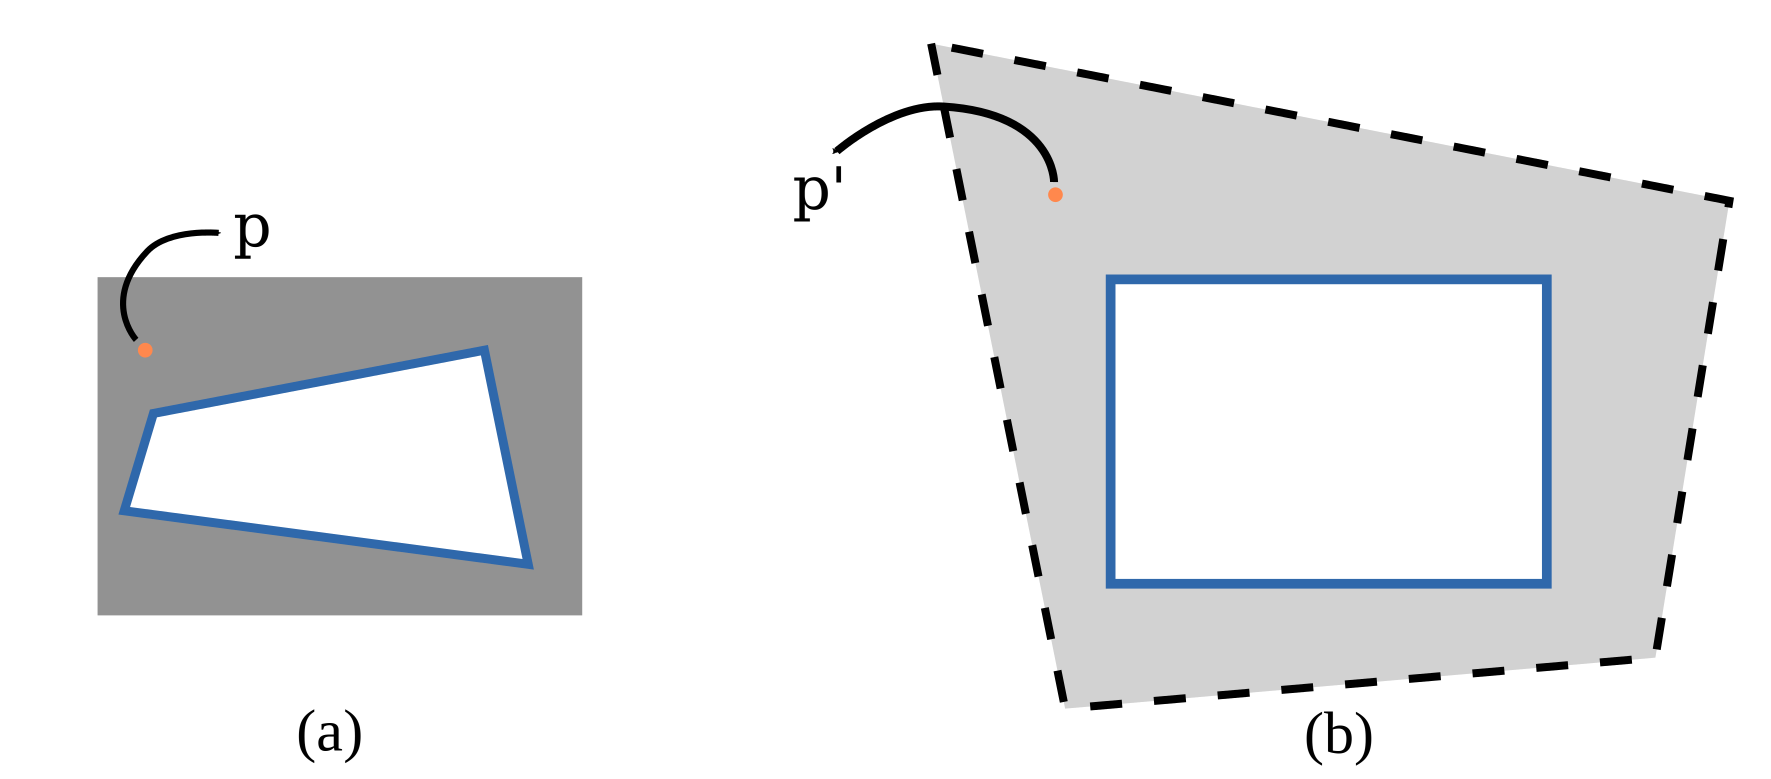
\includegraphics[width=.9\linewidth]{data/result_rect/projection_out_of_bound}
\caption{Diagram of the scenario in which the points in the camera image are mapped outside of the projector image: (a) camera image (b) projector image}
\label{fig:basicModelProjectionOutOfBound}
\end{figure}


A temporary solution to this problem is to reduce the size of the original image by some fixed factor, and place it in the center of the potential (target) camera image, which is some estimate/guess of where the projection lands in the camera image. 
If the scale factor is small enough, this solution would work for most projector-camera arrangements.
However, this method does not guarantee that the anamorph fits inside the projector image for all possible projector and camera positions, and might significantly decrease the size of the resulting anamorphic image.
We will describe a better solution to this problem in the Improved Model discussed in the next section~(\ref{sec:improveModel}).


%\subsection{Results}
%\label{ssec:basicModelResults}





\subsection{Challenges and Limitations}
\label{ssec:basicModelLimitations}

As explained in Subsection \ref{ssec:basicModelGeneratingAnamorph}, the current algorithm for generating the anamorphic image might produce an image that does not fit inside the projector image. An example of this is shown in Figure \ref{fig:basicModelErrorAnamorphOutBound}.

\begin{figure}[ht]
	\centering
	\begin{subfigure}{.45\textwidth}
		\centering
		\shadowimage[width=\linewidth]{data/result_rect/error/error_anamorph}
		\caption{}
		%\label{fig:basicModelAnamorph}
	\end{subfigure} \qquad
	\begin{subfigure}{.45\textwidth}
		\centering
		\shadowimage[width=\linewidth]{data/result_rect/error/error_check_anamorph}
		\caption{}
		%\label{fig:basicModelAnamorph}
	\end{subfigure}
	\caption{(a) Anamorphic image not fitting inside the projector image. (b) When the anamorphic image in (a) is projected, the camera receives an incomplete image.}
	\label{fig:basicModelErrorAnamorphOutBound}
\end{figure}

Figure \ref{fig:basicModelErrorCorners} shows an example of incorrectly detected projection corners, which prevented the program from generating a correct anamorphic image. This error might be caused by poor lighting of the system, which affects the contrast between the projection and the projection surface, making it less detectable by the corner detection function. In some situations, the projection corners are not detected due to the position of the camera, which might be at an angle relative to the projection such that some parts of the projection do not appear clearly in the camera image. 
%1. Lighting: corners not detected correctly - because the contrast in the color intensity between the projection and the projection surface is not large enough. \\
%2. Angle of camera and projection: corners not detected correctly \\
%3. anamorph not fitting inside the projector image.


\begin{figure}[ht]
	\centering
	\shadowimage[width=.7\linewidth]{data/result_rect/error/error_corners}
	\caption{Incorrectly detected projection corners.}
	\label{fig:basicModelErrorCorners}
\end{figure}




%\begin{figure}[ht]
%\centering
%\shadowimage{<Path+filename>}
%\caption{<Caption>}
%\label{<Figure Label>}
%\end{figure}







%%%%%%%%%%%%%%%%%%%%%%%%%%%%%%%%%%%%%%%%%%%%%
%%%   S E C T I O N   %%%%%%%%%%%%%%%%%%%%%%%%%%%%%%%%%
%%%%%%%%%%%%%%%%%%%%%%%%%%%%%%%%%%%%%%%%%%%%%

\section{Improved Planar Model} % Improved Planar Anamorphosis Model
\label{sec:improveModel}
The Basic Model described in the previous section (\ref{sec:basicModel}) presents a simple method for generating an anamorphic image based solely on the homography between the projector and camera image. While effective and sufficient in the simple scenario of our project, the said method has three major limitations. 
First, it neglects the relationship between the physical projection surface to the virtual projector and camera images. Although this missing relationship does not affect the process of generating the anamorphic images when using a camera as the viewer, it is necessary for potential future directions of this project. In particular, the homographies mapping to the projection surface are crucial if we want to generate an anamorphosis for a real person as the viewer instead of the camera, and allow us to easily adapt this system to create a keystone correction model. 
Second, the previous method also fails to reliably eliminate the case of the anamorphic image not fitting inside the projector image. 
Lastly, the pattern detection method described in Subsection \ref{ssec:basicModelPatternDetection} is deficient because it supplies only four point correspondences, which is the minimum number of correspondences required to estimate the homography $H_{PC}$. When the conditions such as lighting, and projector and camera angle are unfavorable, this limitation hinders the process of homography estimation because the error from detecting each of the four corners of the rectangular pattern projected has a significant effect on the accuracy of the resulting homography.
This section uses a modified set-up to incorporate the projection surface, proposes a more complex pattern detection algorithm, and introduces a method for repositioning of the pre-anamorph to guarantee that it fits inside the projector image after warping. 

%TODO resize
\begin{figure}[H]
	\centering
	\begin{subfigure}{.45\textwidth}
		\centering
		\shadowimage[width=.9\linewidth]{data/improvedModel/chessCorners}
		\caption{}
	\end{subfigure}
%	\begin{subfigure}{.4\textwidth}
%		\centering
%		\shadowimage[width=.9\linewidth]{data/improvedModel/max_rect}
%		\caption{}
%	\end{subfigure}
	\begin{subfigure}{.45\textwidth}
		\centering
		\shadowimage[width=.9\linewidth]{data/improvedModel/pre_anamorph}
		\caption{}
	\end{subfigure}
	\begin{subfigure}{.45\textwidth}
		\centering
		\shadowimage[width=.9\linewidth]{data/improvedModel/anamorph}
		\caption{}
	\end{subfigure}%
	\begin{subfigure}{.45\textwidth}
		\centering
		\shadowimage[width=.9\linewidth]{data/improvedModel/check_anamorph}
		\caption{}
	\end{subfigure}%
	\caption{Screenshots of the program: (a) Detected chessboard corners. (b) Prepared pre-anamorph. (c) Anamorphic image after warping. (d) Anamorphic image seen correctly by the camera.}
	%(b) Maximal rectangle that fits inside the projection area.
	\label{fig:resultImproved}
\end{figure}

The modified algorithm is outlined below:
\begin{enumerate}
	\item Project a chessboard pattern.
	\item Find the inner corners of the chessboard in the projector and camera image.
	\item Estimate the homography $H_{PC}$ using the least squares method.
	\item Prepare (resize and reposition) the pre-anamorph.
	\item Generate the anamorph by warping the pre-anamorph with the homography $H_{CP}~=~H_{PC}^{-1}$.
\end{enumerate}
The result of this algorithm is compiled in Figure \ref{fig:resultImproved} and explained in detail later in this section.




%%%%%%%%%%%%%%%%%%%%%%%%%%%%%%%%%%%%%%




\subsection{Modified Set-up}
\label{ssec:improvedModelModifiedSetup}
%TODO check if the fact that "we need to have at least four common points on both surfaces in order to compute the homography between two surfaces" is in that definition that I refered.
We modify our setup to make it possible to find the homographies mapping to the projection surface. 
The Basic Model in Section \ref{sec:basicModel} does not compute any homography involving the projection surface, so there is no need for the projection surface to have any detectable points. In fact, as seen in some camera captures of that model, for example Figures \ref{fig:basicModelCorners} and \ref{fig:basicModelCheckAnamorph}, the projection surface is simply a large blank planar surface, and it is desirable that the the surface does not have any distinguishable features as they could be mistaken by the program for the corners of the projected rectangle that we need to detect. 
However, the new setup introduced in this section requires that the projection surface has some detectable features to facilitate the process of finding the homography mapping to it. We add a rectangular projection surface, on which we project images with the projector. We use a large rectangular piece of paper attached to a wall. The entire projection surface is then captured by the camera, so that the corners of the projection surface can be detected in the camera image.
To find the homography $H_{SC}$ from the projection surface to the camera image, we use the same homography estimation method as the one used to estimate the projector-camera homography $H_{PC}$.


%<picture of the setup>
%<diagram of the setup>


%\begin{figure}[ht]
%\centering
%\shadowimage{<Path+filename>}
%\caption{<Caption>}
%\label{<Figure Label>}
%\end{figure}


\subsection{Detecting the Projection Screen}
\label{ssec:improvedModelProjectionScreen}

We use the same good features to track algorithm to detect the corners of the projection screen. Unlike the projection (light from the projector), the screen is a solid object and its color is appears stable in the camera, which means that the difference in color intensity between the projection screen and the background is more easily detectable than that between the projection and the background. Therefore the Good Features to Track algorithm, described in Section~\ref{ssec:goodFeaturesToTrack}, is relevant as it provides a convenient way to detect exactly four corners of the projection surface. The detected corners are presented in Figure~\ref{fig:improvedModelScreenCorners}.


\begin{figure}[ht]
\centering
%\shadowimage[width=.4\linewidth]{data/improvedModel/screen_corners}
\shadowimage[width=.6\linewidth]{data/improvedModel/screen_corners}
\caption{Detected projection screen corners marked with blue dots.}
\label{fig:improvedModelScreenCorners}
\end{figure}

These corners in the camera image correspond to the corners of the projection surface in the real world. Using these four point correspondences, we can find the homography $H_{SC}$ by using the estimation method described in Subsection~\ref{ssec:leastSqHomograph}, where the real-world corners of the projection surface assume the role of the projector points in the estimation method, and the detected corners of the surface in the camera image are the output points..

%Note that $H_{SC}$ could also be found for example if we stick a poster card on the wall, and detect it in the camera.






\subsection{Homography Estimation with Chessboard Corner Detection}
\label{ssec:improvedModelChessDetect}
%chessboard detection for H_PC

The Basic Model described in Section~\ref{sec:basicModel} uses a simple corner detection function to find the corners of a rectangular shape projected on a wall, as seen in the camera image (Figure~\ref{fig:basicModelCorners}), and matches these corners with the corners of the original shape that was projected, as seen on the computer screen. These four corner correspondences are then used to find the homography $H_{PC}$. This method requires a specific light setting, and might not produce the desired results when the light is too bright as the projection might not be clearly visible in the camera image.

\begin{figure}[h]
	\centering
	\begin{subfigure}{.47\textwidth}
		\centering
		\shadowimage[width=\linewidth]{data/improvedModel/chessboard}
		\caption{}
		\label{fig:improvedModelChess}
	\end{subfigure} \qquad
	\begin{subfigure}{.47\textwidth}
		\centering
		\shadowimage[width=\linewidth]{data/improvedModel/chessCorners}
		\caption{}
		\label{fig:improvedModelChessDetected}
	\end{subfigure}
	\caption{(a) Original chessboard corners in the projector image. (b) Detected chessboard corners in the camera image.}
	\label{fig:improvedModelChessCorners}
\end{figure}

This subsection introduces an alternative way to obtain points in the projector and camera image that provide a better estimation of the homography $H_{PC}$. The major amendment is in the pattern projected. Instead of the simple rectangular pattern that contains only four detectable features, we project a $6\times 9$ chessboard pattern, presented in Figure~\ref{fig:improvedModelChess}, with $5\cdot 8 = 40$ detectable inner corners. We choose this pattern because it is easily distinguishable from the projection screen. Notice that if we repeat the pattern detection process from the Basic Model (Section~\ref{sec:basicModel}), the algorithm used to detect the projection corners might not be able to distinguish between the corners of the projection and the projection surface. The chessboard provides an efficient solution because it can be easily detected regardless of other detectable objects surrounding it in the camera image, as shown in Figure~\ref{fig:improvedModelChessDetected}. 
%We use the chessboard detection method described in Subsection~\ref{ssec:chess}.

% Why chessboard is better here and more relevant. -> Because in this model we include a separate screen (projection screen, which is a large rectangular sheet of paper), the screen itself has detectable corners that could be wrongly detected as the features for our pattern matching. Therefore the pattern needs to be unique and easily distinguishable from the projection screen corners.




\subsection{Repositioning and Resizing the Pre-anamorph}
\label{ssec:improvedModelReshapePreAnamorph}
% max_rect

A major limitation of the Basic Model is the fact that the anamorph may not fit entirely within the projector image after warping. Recall that this phenomenon occurs because the entire projector image is mapped by $H_{PC}$ into an area inside the camera image. It follows that the inverse homography $H_{CP}$ maps the points within that projection area (inside the camera image) back to their positions in the projector image. However, the points in the camera image that lie outside of the projection area are mapped to new positions that do not fit inside the projector image, as illustrated in Figure~\ref{fig:basicModelProjectionOutOfBound}.

We propose a method for resizing and repositioning the pre-anamorph before warping it to ensure that the resulting anamorph fits entirely inside the projector image and is of the largest size possible, described in the following steps:
\begin{enumerate}%[itemsep=0mm]%\singlespace
	\item Identify the four corners of the quadrilateral region of the projection area inside the camera image by applying $H_{PC}$ to each of the four outer corners of the projection image. The detected projection is shown in Figure~\ref{fig:improvedModelProjectionBounds}.
	\item Find the largest rectangle that fits inside the projection region in the camera image, as shown in Figure~\ref{fig:improvedModelMaxRect}. We explain this in more detail below.
	\item Resize the original image so that it fits inside that rectangle, and place it in a blank (uniformly colored) camera image in a position that is aligned with the position of that rectangle (for example by aligning the top-left corner of the pre-anamorph with the top-left corner of that rectangle), as shown in Figure~\ref{fig:improvedModelPreAnamorphPrepared}.
\end{enumerate}
After accomplishing these steps, the pre-anamorph is ready to be warped and is ensured to land inside the projector image.

\begin{figure}[t]
	\centering
	\begin{subfigure}{.47\textwidth}
		\centering
		\shadowimage[width=\linewidth]{data/improvedModel/projectionInCameraCorners}
		\caption{Corners of the projection area in the camera image.\\}
		\label{fig:improvedModelProjectionBounds}
	\end{subfigure} \qquad
	\begin{subfigure}{.47\textwidth}
		\centering
		\shadowimage[width=\linewidth]{data/improvedModel/max_rect}
		\caption{Maximal rectangle with fixed aspect ratio that fits inside the projection area.\\}
		\label{fig:improvedModelMaxRect}
	\end{subfigure} \qquad
	\begin{subfigure}{.47\textwidth}
		\centering
		\shadowimage[width=\linewidth]{data/improvedModel/pre_anamorph}
		\caption{Prepared pre-anamorph.}
		\label{fig:improvedModelPreAnamorphPrepared}
	\end{subfigure}
	\caption{Screenshots of the program}
	\label{fig:improvedModelPreparePreAnamorph}
\end{figure}

It remains to explain the method for finding the largest rectangle inside a quadrilateral figure. Our method iterates through the pixels in the camera image and searches for the largest rectangle that fits inside the projection area. We improve the run-time of the algorithm by iterating only through the pixels that lie inside the projection area, before searching for the best rectangle, and we stop the iteration once the remaining area in the camera image is smaller than the current largest rectangle. Additionally, we require that the rectangle has the same aspect ratio as the original image. 

%{\color{red}pseudocode of how max rect is computed in appendix}





\subsection{Challenges and Limitations}
\label{ssec:improvedModelLimitations}

One minor issue we encounter when testing this model is that for some positions of the camera, the chessboard pattern is not detected correctly. One possible explanation is that the camera is at an angle (relative to the projection screen) such that the chessboard pattern appears too small, which causes the chessboard corners to be too crowded to be detected correctly. In addition, the projector light is not stable, which reduces the quality of the camera picture and makes it more difficult to accurately detect the chessboard corners.
However, none of the tests performed have shown a noticeable deterioration in the quality of the anamorphic image. Because the number of chessboard corners is significantly larger than four, which is the minimum number of points required to establish a homography, the inaccuracy in detecting some of them is less likely to significantly affect the final result.



\begin{figure}[ht]
\centering
\shadowimage[width=.7\linewidth]{data/improvedModel/error/chessCornersError}
\caption{A scenario in which the program fails to detect the chessboard corners correctly.}
\label{fig:improvedModelChessError}
\end{figure}










%%%%%%%%%%%%%%%%%%%%%%%%%%%%%%%%%%%%%%%%%%%%%
%%%   S E C T I O N   %%%%%%%%%%%%%%%%%%%%%%%%%%%%%%%%%
%%%%%%%%%%%%%%%%%%%%%%%%%%%%%%%%%%%%%%%%%%%%%

%\section{Keystone Correction}
%\label{sec:keystoneImplement}
























%%%%%%%%%%%%%%%%%%%%%%%%%%%%%%%%%%%%%%%%%%%%%
%%%   S E C T I O N   %%%%%%%%%%%%%%%%%%%%%%%%%%%%%%%%%
%%%%%%%%%%%%%%%%%%%%%%%%%%%%%%%%%%%%%%%%%%%%%

\section{Two-view Anamorphosis}
\label{sec:2view}

%TODO where is this definition?
By the definition of anamorphosis, there is only one perspective, or rather one ray, such that when a viewer looks at the anamorphic image from any point on that ray, the anamorphic image appears as the original unwarped image to the viewer. However, in practice there might be a number of viewers looking at the anamorphic image from several perspectives. In this section we address this issue and test a method for finding a transformation that minimizes the distortions for the viewers. Once again, we use cameras to represent viewers, and assume that the camera captures are what the viewers observe. Our goal is to produce a homography $\widehat{H}$ such that when $\widehat{H}$ is applied to an image, and the resulting anamorphic image is projected onto the projection surface, each camera capture of the projected image is ``as close as possible" to the original unwarped image. Strictly following the definition of anamorphosis, the image transformed with that homography is not an anamorphosis for any of the cameras, because an anamorphosis can satisfy only one perspective. Rather than generating an image that is an anamorphosis for all the viewers, which is theoretically impossible, we aim to generate an image that is ``as close as possible" to the anamorphosis for each viewer. Although the result of this program is not an anamorphic image,  for consistency, we continue to use the terms ``pre-anamorph" and ``anamorph" to refer to the unwarped image and the final warped image that is projected, respectively.

The first question we need to answer is: how do we define ``closeness" between the desired image and the actual image we obtain? In other words, what is the error? One way to define it is in terms of distance, which in this scenario means the distance between the same pixel in the two images in the $x$ and $y$ direction. 
%For example, if the pixel at position $(3, 4)$ from the original image lands at position $(5,10)$ in one image, and $(9,2)$ in the other, then the distance between the two images at that pixel is $4$ in the $x\text{-direction}$, and $-8$ in the $y\text{-direction}$. 
We take the sum of the squared distances at each pixel as a measure of the error between the obtained and target image. Based on this definition, our reformulated goal is to find a homography such that when it is applied to an image, and the image is projected on the projection surface, and then captured by the two cameras, the sum of the errors between the captures and the desired images is minimized. This problem is different from the previous two models in Sections \ref{sec:basicModel} and \ref{sec:improveModel} in that we need to minimize the error for both camera images, which makes the estimation of the optimal homography to warp the original image to the projector image significantly more complex.

The inclusion of the second camera requires that we introduce some changes to the program. We present the updated outline of the algorithm to generate an optimal image for two viewers:
\begin{enumerate}
	\item Project a chessboard pattern.
	\item Find the inner corners of the chessboard in Camera 1 and Camera 2 images.
	\item Estimate the projector-camera homography for each camera, using the same method as in the Improved Model in Section \ref{sec:improveModel}.
	\item Choose a target chessboard pattern for each camera.
	\item Estimate the homography $\widehat{H}$ and its inverse $\widehat{H}^{-1}$ that map between the original image and the projector image, and minimize the difference in the observed chessboard corners and the target chessboard corners for each camera. The new homography notation is explained in the following Subsection \ref{ssec:2viewSetup}.
	\item Prepare (resize and reposition) the pre-anamorph.
	\item Generate the anamorph by warping the pre-anamorph with the homography $\widehat{H}^{-1}$.
\end{enumerate}



\subsection{Two-view Setup}
\label{ssec:2viewSetup}

The equipment needed for this setup is a projector, and projection surface, and two cameras. As in the previous models, we require that the projector and the cameras are directed towards the projection screen, and that the images projected land inside the projection screen, and the cameras capture the entire projection screen. This setup is visualized in Figure \ref{fig:2viewSetup}.
%[width=.4\linewidth]

\begin{figure}[ht]
\centering
\includegraphics[width=.7\linewidth]{data/2view/setup/setup2short2}
\caption{The new setup: (a) Camera 1 (b) Projector (c) Camera 2 (d) Projection surface.}
\label{fig:2viewSetup}
\end{figure}

Along with the changed setup, we also introduce a new notation of the homographies for this particular two view model, as presented in Figure \ref{fig:2viewHDiagram}. We denote the homography from the projector image to the first camera image as $A$, and the homography from the projector image to the second camera image as $B$. $A$ and $B$ correspond to the projector-camera homography $H_{PC}$ from the one view models discussed earlier. 
We introduce a new homography $\widehat{H}$ from the projector image to the original image. It follows that the inverse homography $\widehat{H}^{-1}$ maps from the original image to the projector image, and that $A\widehat{H}^{-1}$ and $B\widehat{H}^{-1}$ map from the original image to the first and second camera image respectively. 
Recall that the previous one-view models use the homography $H_{CP}$ to warp the pre-anamorph into the anamorph. This method stems from the valid assumption that the pre-anamorph is the target camera image, and the anamorph is the projector image, so the anamorph can be created by warping the target camera image into the projector image. 
However, this approach is not applicable to this model because the homography used to warp the pre-anamorph into the anamorph is neither $A^{-1}$ (the camera-projector homography for camera 1) nor $B^{-1}$ (the camera-projector homography for camera 1). In fact, if either $A^{-1}$ or $B^{-1}$ is used to create the anamorph, the result will be optimized for only one of the cameras. 
Therefore, this model requires a new homography $\widehat{H}$ to optimize the projected image for both camera views. 
The primary task in this model is to estimate the best homography $\widehat{H}$ as we need it to warp the original image (pre-anamorph) into the optimal anamorphic image, which is then projected.

\begin{figure}[t]
	\centering
	\includegraphics[width=.7\linewidth]{data/2view/setup/2view_Hdiagram}
	\caption{The new setup and notation for the homographies.}
	\label{fig:2viewHDiagram}
\end{figure}


\subsection{Target Camera Images}
\label{ssec:2viewTargetCamera}

The steps 1 through 3 outlined at the beginning of this section give an estimate of the homographies $A$ and $B$ using the estimation method described in the previous one-view models. It remains to determine the homography $\widehat{H}$. Before we introduce the new method for homography estimation, we reiterate the approach used in the previous models to explain why it does not apply in the current two-view model, which sheds some light on the modifications we need to make to adapt the previous method to this scenario.

%The approach of homography estimation used in the previous models 
In the Improved Model approach, we project a chessboard pattern and detect the transformed chessboard corners in the camera image, as explained in Subsection~\ref{ssec:improvedModelChessDetect}. We then investigate the relationship between the original chessboard corners (in the projector image) and those detected in the camera image, and find the best homography $H_{PC}$ that transforms the original chessboard points to the camera points. The reason why this method can only be used to estimate the homographies $A$ and $B$, but cannot be used to estimate the homography $\widehat{H}$ is that the previous approach considers the relationship of points between the projector and camera image, while
$\widehat{H}$ relates points between the projector image and the original image (or the pre-anamorph). 

To address this issue, we introduce a new estimation approach, which allows us to solve for the best homographies $AH^{-1}$ and $BH^{-1}$ between the original image and the camera image. Because $A$ and $B$ are already known to us from the earlier steps of the program, we effectively solve for $H^{-1}$. To do this, we need a set of points in the original image, and a corresponding set of points in each camera image. The points on the original image are simply the original chessboard corners. The target points on each camera image are the same as the original chessboard points, up to scale and translation. This follows from the reasoning that when the original image is the pre-anamorph (i.e. the picture that we use to generate the final anamorphic image), our goal is for the cameras to see the same picture as the original image, up to scale and translation.

To account for the location of the actual projection in each camera image, we find the new chessboard corners by performing a least squares minimization on the detected chessboard corners. In addition, we impose the following constraints on the new chessboard pattern:
\begin{enumerate}
	\item The number of rows and columns in the new pattern is the same as that of the original chessboard pattern.
	\item The chessboard corners are equally spaced.
	\item The grid lines of the new pattern are parallel to the $x$ and $y$ axes.
\end{enumerate}
The result of this method is presented in Figure \ref{fig:2viewNewChess}

\begin{figure}[H]
	\centering
	\begin{subfigure}{.47\textwidth}
		\centering
		\shadowimage[width=\linewidth]{data/2view/newChess1}
		\caption{New chessboard pattern for Camera 1 shown with red dots.}
		\label{fig:2viewNewChess1}
	\end{subfigure} \qquad
	\begin{subfigure}{.47\textwidth}
		\centering
		\shadowimage[width=\linewidth]{data/2view/newChess2}
		\caption{New chessboard pattern for Camera 2 shown with red dots.}
		\label{fig:2viewNewChess2}
	\end{subfigure}
	\caption{New chessboard patterns.}
	\label{fig:2viewNewChess}
\end{figure}



\subsection{Homography Estimation}
\label{ssec:2viewHomography}

Due to the changes in the setup, the homography estimation method used in the previous models no longer applies. Therefore, we introduce a homography estimation method designed specifically for this model. While this technique bears some similarities to the previous method in that we continue to use the least squares minimization to find the optimal homography $\widehat{H}$, the function that we minimize on is significantly different. This subsection provides a detailed explanation of the new homography estimation using the homogeneous least squares for the two view model.

%TODO define all the variables here:
Let $p_0, p_1, \dots, p_{n-1}$ be the chessboard corners in the original image. Let $v_0, v_1, \dots, v_{n-1}$ and $w_0, w_1, \dots, w_{n-1}$ be the target chessboard corners in Camera 1 and Camera 2 respectively. The homography that maps points from the original image to a camera image is $A\widehat{H}^{-1}$ for Camera 1 and $B\widehat{H}^{-1}$ for Camera 2, where the entries of $\widehat{H}^{-1}$ are the unknowns. Let $h_{00}, h_{01}, \dots, h_{22}$ be the entries of $ \widehat{H}^{-1} $ so that
\[
\widehat{H}^{-1} = 
\begin{bmatrix}
h_{00} & h_{01} & h_{02} \\
h_{10} & h_{11} & h_{12} \\
h_{20}& h_{21} & h_{22}
\end{bmatrix}.
\]
Without loss of generality, we assume that $h_{22} = 1$. By the homogeneous least squares described in Subsection \ref{ssec:hEstimateHomogeneousLS}, the error function $E$ can be defined as:
\begin{align*}
E(h_{00}, h_{01}, \dots, h_{21}, \lambda_0, \lambda_1, \dots, \lambda_{n-1}, \mu_0, \mu_1, \dots, \mu_{n-1}) 
= &\sum_{k=0}^{n-1} \left(  \left\| A\widehat{H}^{-1}p_k - \lambda_k v_k\right\|^2 \right)\\
+ &\sum_{k=0}^{n-1} \left( \left\|B\widehat{H}^{-1}p_k - \mu_k w_k\right\|^2 \right)
\end{align*}
for some scaling variables $\lambda_k$ corresponding to each target point $v_k$ in Camera 1, and $\mu_k$ corresponding to each target point $w_k$ in Camera 2. 
The scaling factors account for the fact that any multiple of a homogeneous point corresponds to the same point, and so taking the difference between $A\widehat{H}^{-1}p_k$ and a multiple of $v_k$, and the difference between $B\widehat{H}^{-1}p_k$ and a multiple of $w_k$ gives a better estimate of the actual distance between these pairs of points than, for example taking the difference of $A\widehat{H}^{-1}p_k$ and unscaled $v_k$.

Observe that $\left\| A\widehat{H}^{-1}p_k - \lambda_k v_k\right\|$ and $\left\|B\widehat{H}^{-1}p_k - \mu_k w_k\right\|$ are of similar structure, which allows us to rewrite the error function in an equivalent but simpler form:
\[
E(X_{00}, X_{01}, \dots, X_{21}, \sigma_0, \sigma_1, \dots, \sigma_{2n-1}) 
= \sum_{k=0}^{2n-1} \left\| A_k X b_k - \sigma_k c_k\right\|^2
\]
where $A_k$ is $A$ or $B$, $X$ is $\widehat{H}^{-1}$, $b_k$ is $p_{k-n}$, $\sigma_k$ is $\lambda_k$ or $\mu_{k-n}$, and $c_k$ is $v_k$ or $w_{k-n}$, depending on the value of $k$, as shown in Table \ref{fig:errorVarMeaning}.
\begin{table}[ht]
\renewcommand{\arraystretch}{1.5}
\centering
	\begin{tabular}{ l || c | c | c | c | c }
		& $A_k$ & $X$ & $b_k$ & $\sigma_k$ & $c_k$ \\ \hline
		\hline
		$0 \le k \le n-1$ & $A$ & $\widehat{H}^{-1}$ & $p_k$ & $\lambda_k$ & $v_k$ \\ \hline
		$n \le k \le 2n-1$ & $B$ & $\widehat{H}^{-1}$ & $p_{k-n}$ & $\mu_{k-n}$ & $w_{k-n}$ \\
	\end{tabular}
	\caption{The meaning of new variables $A_k, X, b_k, \sigma_k$ and $c_k$.}
	\label{fig:errorVarMeaning}
\end{table}

The goal of this section is to find $(h_{00}, h_{01}, \dots, h_{21}, \sigma_0, \sigma_1, \dots, \sigma_{2n-1})$ that minimize the error function. As explained in Section \ref{sec:leastSquares}, we find partial derivatives of $E$ with respect to each variable, and solve a system of linear equations in which each partial derivative is zero. For simplicity, we perform the differentiation on the simple form of the error function. The solution to that system of equations is the vector $(X_{00}, X_{01}, \dots, X_{21}, \sigma_0, \sigma_1, \dots, \sigma_{2n-1})$. In particular, the values $X_{00}, X_{01}, \dots, X_{21}$ in the solution are the entries of the homography matrix $\widehat{H}^{-1}$.

The partial derivatives take two different forms depending on the variable with respect to which we differentiate. We distinguish these two types of variables: $X_{rs}$ where $0 \le r,s \le 2$, and $\sigma_r$ where $0 \le r \le 2n-1$.

The partial derivative of $E$ with respect to $X_{rs}$ for any $r,s$ such that $0 \le r,s \le 2$ is:
\begin{align}
\frac{\partial}{\partial  X_{rs}} & \sum_{k=0}^{2n-1} \left\| A_k X b_k - \sigma_k c_k \right\|^2 \nonumber\\
&= 2\sum_k \left(A_k X b_k - \sigma_k c_k\right) \cdot \left(A_k E_{rs}b_k\right) \label{eq:2viewDeriv1} \\
&= 2\sum_k \sum_{l} \left(A_k X b_k - \sigma_k c_k\right)_l \left(A_k E_{rs}b_k\right)_l \label{eq:2viewDeriv2} \\
&= 2\sum_k \sum_l 
\left( \left(A_k X b_k\right)_l - \sigma_k \left(c_k\right)_l \right)
\left(\left(A_k\right)_{lr} \left(b_k\right)_s\right) \label{eq:2viewDeriv3} \\
&= 2 \sum_k \sum_l
\left( \left(\sum_{i,j}\left(A_k\right)_{li} X_{ij}\left(b_k\right)_j \right) - \sigma_k \left(c_k\right)_l \right) 
\left(\left(A_k\right)_{lr} \left(b_k\right)_s \right) \label{eq:2viewDeriv4} \\
&= 2\left( 
\sum_{i,j} \sum_k\sum_l \left(A_k\right)_{li} \left(b_k\right)_j \left(A_k\right)_{lr} \left(b_k\right)_s X_{ij} 
- \sum_k \sum_l \left(c_k\right)_l \left(A_k\right)_{lr} \left(b_k\right)_s \sigma_k 
\right). \nonumber
\end{align}

The $E_{rs}$ in lines (\ref{eq:2viewDeriv1}) and (\ref{eq:2viewDeriv2}) of the derivation above is defined as a matrix with one at the position $rs$, and zero everywhere else.
For aesthetic purposes we skip the bounds on the sums in the derivation above, and explain them here. The index iterator $l$ results from taking the dot product of $A_k X b_k - \sigma_k c_k$ and $A_k E_{rs}b_k$, each of which are vectors of length 3, therefore $0 \le l \le 2$. The index iterators $i$ and $j$ result from taking the $l^{th}$ entry of the product of $A_k$, $X$ and $b_k$. Since $A_k$ and $X$ are $3 \times 3$ matrices, and $b_k$ is a vector of length 3, it follows that $0 \le i,j \le 2$. 
From (\ref{eq:2viewDeriv1}) to (\ref{eq:2viewDeriv2}), we use the fact that the dot product of two vectors $\vec{u}$ and $ \vec{v}$ is $\vec{u}\cdot \vec{v} = \sum_l u_l v_l$.
From (\ref{eq:2viewDeriv2}) to (\ref{eq:2viewDeriv3}) we use the following derivation:
\begin{align*}
\left(A_kE_{rs}b_k\right)_l 
&= \left(A_k(E_{rs}b_k)\right)_l \\
&= \left(A_k\left(0,\dots,(b_k)_s,\dots,0\right)^T\right)_l \text{, where } (b_k)_s \text{ is the } r^{th} \text{ entry}\\
&= (A_k)_{lr}(b_k)_s.
\end{align*}
From (\ref{eq:2viewDeriv3}) to (\ref{eq:2viewDeriv4}) we use these two properties:
\[\left(A\vec{v}\right)_l = \sum_i A_{li}v_i, \text{ and}\]
\[ \left(AB\vec{v}\right)_l
= \sum_i A_{li}(B\vec{v})_i 
= \sum_i \left( A_{li} \sum_j B_{ij}v_j \right) 
= \sum_{ij} A_{li}B_{ij}v_j. \]

We set this derivative to zero, and rearrange it so that the constant terms are on the right-hand side. Because $X_{22} = 1$, the term $X_{22}$ and its coefficients are moved to the right-hand side:
\begin{align}
 2\left( 
\sum_{i,j} \sum_{k}\sum_{l} \left(A_k\right)_{li} \left(b_k\right)_j \left(A_k\right)_{lr} \left(b_k\right)_s X_{ij} 
- \sum_k \sum_l \left(c_k\right)_l \left(A_k\right)_{lr} \left(b_k\right)_s \sigma_k 
\right) &= 0 \nonumber\\
 \sum_{i,j} \sum_k\sum_l \left(A_k\right)_{li} \left(b_k\right)_j \left(A_k\right)_{lr} \left(b_k\right)_s X_{ij} 
- \sum_k \sum_l \left(c_k\right)_l \left(A_k\right)_{lr} \left(b_k\right)_s \sigma_k &= 0 \nonumber\\
 \sum_{(i,j) \not= (2,2)} \sum_k\sum_l \left(A_k\right)_{li} \left(b_k\right)_j \left(A_k\right)_{lr} \left(b_k\right)_s X_{ij} 
- \sum_k \sum_l \left(c_k\right)_l \left(A_k\right)_{lr} \left(b_k\right)_s \sigma_k & \nonumber\\
 = \sum_k\sum_l \left(A_k\right)_{l2} \left(b_k\right)_2 \left(A_k\right)_{lr} \left(b_k\right)_s. \label{eq:2viewDeriv1Done}
\end{align}

Converting the equation (\ref{eq:2viewDeriv1Done}) back to the notation used in our initial setup of this model, we have the following equation:
\begin{align*}
&\sum_{(i,j) \not= (2,2)} 
\left[
\sum_k \sum_l A_{li}(p_k)_jA_{lr}(p_k)_s + B_{li}(p_k)_jB_{lr}(p_k)_s
\right] h_{ij} \\
&- \sum_k
\left[ 
\sum_l (v_k)_l A_{lr} (p_k)_s
\right] \lambda_k \\
&- \sum_k \left[
\sum_l (w_k)_l B_{lr} (p_k)_s
\right] \mu_k \\
= &- \sum_k \sum_l 
\left[
A_{l2}(p_k)_2 A_{lr} (p_k)_s +
B_{l2}(p_k)_2 B_{lr} (p_k)_s
\right].
\end{align*}


The partial derivative with respect to $\sigma_r$ for any $0 \le r \le 2n-1$ is:
\begin{align*}
\frac{\partial}{\partial \sigma_r} & \sum_{k=0}^{2n-1} \left\| A_k X b_k - \sigma_k c_k \right\|^2 \\
& = \frac{\partial}{\partial \sigma_r} \left\| A_r X b_r - \sigma_r c_r \right\|^2 \\
& = -2 \left(
A_r X b_r - \sigma_r c_r
\right)
\cdot c_m \\
& = -2 \sum_l \left(
A_r X b_r - \sigma_r c_r
\right)_l
\left(c_r\right)_l \\
& = -2 \sum_l \left(
\left(
\sum_{i,j} \left(A_r\right)_{li} X_{ij} \left(b_r\right)_j
\right)
- \sigma_r \left(c_r\right)_l
\right)
\left(c_r\right)_l \\
& = -2 \left(
\sum_{i,j} \sum_l
\left(A_r\right)_{li} \left(b_r\right)_j \left(c_r\right)_l X_{ij}
-
\sum_l 
\left(c_r\right)_l^2 \sigma_r
\right).
\end{align*}

Notice that in the process of taking the derivative, the summation on $k$ disappeared. This is because $\frac{\partial}{\partial \sigma_r} \left\| A_k X b_k - \sigma_k c_k \right\|^2 = 0$ for all $k \not= r$. We explain the limits on the summations above: $l$ is the iterator in the dot product of $A_r X b_r - \sigma_r c_r$ and $c_m$, both of which are vectors of length 3, so $0 \le l \le 2$; $i$ and $j$ are iterators in taking the $l^{th}$ entry of the product of $A_k$, $X$ and $b_k$, and since $A_k$ and $X$ are $3\times 3$ matrices and $b_k$ is a vector of length 3, it follows that $0 \le i,j \le 2$.

Again, we set the derivative to zero and bring the constant terms to the right-hand side:
\begin{align}
-2 \left(
\sum_{i,j} \sum_l
\left(A_r\right)_{li} \left(b_r\right)_j \left(c_r\right)_l X_{ij}
-
\sum_l 
\left(c_r\right)_l^2 \sigma_r
\right) &= 0 \nonumber\\
\sum_{i,j} \sum_l
\left(A_r\right)_{li} \left(b_r\right)_j \left(c_r\right)_l X_{ij}
-
\sum_l 
\left(c_r\right)_l^2 \sigma_r &= 0 \nonumber\\
\sum_{(i,j) \not= (2,2)} \sum_l
\left(A_r\right)_{li} \left(b_r\right)_j \left(c_r\right)_l X_{ij}
-
\sum_l 
\sigma_r \left(c_r\right)_l^2 &= \sum_l
\left(A_r\right)_{l2} \left(b_r\right)_2 \left(c_r\right)_l. \label{eq:2viewDeriv2Done}
\end{align}

Converting to the notation used in our initial setup of this model, we obtain two equations depending on the value $r$. When $0 \le r \le n-1$, $\sigma_r=\lambda_r$, and the equation~(\ref{eq:2viewDeriv2Done})~is
\[
\sum_{(i,j) \not= (2,2)}
\left[
\sum_l A_{li} (p_r)_j (v_r)_l
\right] h_{ij}
- \left[ 
\sum_l (v_r)_l^2
\right] \lambda_r
=
-\sum_l A_{l2}(p_r)_2 (v_r)_l.
\]
When $n \le r \le 2n-1$, $\sigma_r =\mu_{r-n}$ and the equation (\ref{eq:2viewDeriv2Done}) is
\[
\sum_{(i,j) \not= (2,2)}
\left[
\sum_l B_{li} (p_{r-n})_j (w_{r-n})_l
\right] h_{ij}
- \left[ 
\sum_l (w_{r-n})_l^2
\right] \mu_r
=
-\sum_l B_{l2}(p_{r-n})_2 (w_{r-n})_l.
\]
We solve the resulting system of equations for the unknowns $h_{00}, h_{01}, \dots, h_{21}$, $\lambda_0$, $\lambda_1, \dots, \lambda_{n-1}$, $\mu_0, \mu_1, \dots, \mu_{n-1}$, where $h_{00}, h_{01}, \dots, h_{21}$ and $1$ are the entries of the homography~$\widehat{H}^{-1}$.







%\begin{align*}
%&\frac{\partial}{\partial  X_{r,s}} = 0 \\
%& 2\left( 
%\sum_{i,j} \sum_{k}\sum_{l} \left(A_k\right)_{l,i} \left(b_k\right)_j \left(A_k\right)_{l,r} \left(b_k\right)_s X_{i,j} 
%- \sum_k \sum_l \left(c_k\right)_l \left(A_k\right)_{l,r} \left(b_k\right)_s \sigma_k 
%\right) = 0 \\
%& \sum_{i,j} \sum_k\sum_l \left(A_k\right)_{l,i} \left(b_k\right)_j \left(A_k\right)_{l,r} \left(b_k\right)_s X_{i,j} 
%- \sum_k \sum_l \left(c_k\right)_l \left(A_k\right)_{l,r} \left(b_k\right)_s \sigma_k = 0 \\
%& \sum_{(i,j) \not= (2,2)} \sum_k\sum_l \left(A_k\right)_{l,i} \left(b_k\right)_j \left(A_k\right)_{l,r} \left(b_k\right)_s X_{i,j} 
%- \sum_k \sum_l \left(c_k\right)_l \left(A_k\right)_{l,r} \left(b_k\right)_s \sigma_k
%\\
%& = \sum_k\sum_l \left(A_k\right)_{l,2} \left(b_k\right)_2 \left(A_k\right)_{l,r} \left(b_k\right)_s X_{2,2}
%\end{align*}


%\begin{align*}
%	\frac{\partial}{\partial  X_{r,s}} & \sum_{k=0}^{2n-1} \left\| A_k X b_k - \sigma_k c_k \right\|^2 \\
%	&= 2\sum_{k=0}^{2n-1} \left(A_k X b_k - \sigma_k c_k\right) \cdot \left(A_k E_{r,s}b_k\right) \\
%	&= 2\sum_{k=0}^{2n-1} \sum_{l=0}^2 \left(A_k X b_k - \sigma_k c_k\right)_l \left(A_k E_{r,s}b_k\right)_l \\
%	&= 2\sum_{k=0}^{2n-1} \sum_{l=0}^2 
%	\left( \left(A_k X b_k\right)_l - \sigma_k \left(c_k\right)_l \right)
%	\left(\left(A_k\right)_{l,r} \left(b_k\right)_s\right) \\
%	&= 2 \sum_{k=0}^{2n-1} \sum_{l=0}^{2}
%	\left( \left(\sum_{i=0}^2 \sum_{j=0}^2\left(A_k\right)_{l,i} X_{i,j}\left(b_k\right)_j \right) - \sigma_k \left(c_k\right)_l \right) 
%	\left(\left(A_k\right)_{l,r} \left(b_k\right)_s \right) \\
%	&= 2\left( 
%	\sum_{i=0}^{2} \sum_{j=0}^{2} \sum_{k=0}^{2n-1}\sum_{l=0}^{2} \left(A_k\right)_{l,i} \left(b_k\right)_j \left(A_k\right)_{l,r} \left(b_k\right)_s X_{i,j} 
%	- \sum_{k=0}^{2n-1} \sum_{l=0}^{2} \left(c_k\right)_l \left(A_k\right)_{l,r} \left(b_k\right)_s \sigma_k 
%	\right)
%\end{align*}
%
%We set this derivative to be equal to zero, and rearrange it so that the constant terms are on the right-hand side. Because $X_{2,2} = 1$, the term $X_{2,2}$ with its coefficients are moved to the right-hand side:
%\begin{align*}
%& 2\left( 
%\sum_{i=0}^{2} \sum_{j=0}^{2} \sum_{k=0}^{2n-1}\sum_{l=0}^{2} \left(A_k\right)_{l,i} \left(b_k\right)_j \left(A_k\right)_{l,r} \left(b_k\right)_s X_{i,j} 
%- \sum_{k=0}^{2n-1} \sum_{l=0}^{2} \left(c_k\right)_l \left(A_k\right)_{l,r} \left(b_k\right)_s \sigma_k 
%\right) = 0 \\
%& \sum_{i=0}^{2} \sum_{j=0}^{2} \sum_{k=0}^{2n-1}\sum_{l=0}^{2} \left(A_k\right)_{l,i} \left(b_k\right)_j \left(A_k\right)_{l,r} \left(b_k\right)_s X_{i,j} 
%- \sum_{k=0}^{2n-1} \sum_{l=0}^{2} \left(c_k\right)_l \left(A_k\right)_{l,r} \left(b_k\right)_s \sigma_k = 0 \\
%& \sum_{i=0}^{2} \sum_{j=0}^{2} \sum_{k=0}^{2n-1}\sum_{l=0}^{2} \left(A_k\right)_{l,i} \left(b_k\right)_j \left(A_k\right)_{l,r} \left(b_k\right)_s X_{i,j} 
%- \sum_{k=0}^{2n-1} \sum_{l=0}^{2} \left(c_k\right)_l \left(A_k\right)_{l,r} \left(b_k\right)_s \sigma_k =
%\end{align*}










\subsection{Generating the Anamorphic Image}
\label{ssec:2viewGenerateAnamorphicImage}

To generate the anamorphic image, we perform the repositioning and resizing steps described in Subsection \ref{ssec:improvedModelReshapePreAnamorph} in the Improved Model. We then apply the $\widehat{H}^{-1}$ to the prepared pre-anamorph, which lies on the original image, to transform it into the anamorph on the projector image. 

Our initial attempts did not provide expected results prompting us to identify some potential shortcomings in our model. We tested the algorithm for homography estimation using the homogeneous least squares method on specific parameters to verify if the algorithm is correct. We compare the obtained test results with a parallel computation in Mathematica. The results of the tests suggest that the implementation works for parameters that can be expressed with few decimal digits, but does not give the expected solution for parameter with many decimal digits. This finding led us to consider the possibility of encountering ill-conditioned matrices, which are matrices in which the difference in between the smallest and largest entries is large, which causes the program to lose some accuracy when performing Gaussian elimination on those numbers. Further tests confirmed this conjecture as the condition number was between 4 and 10, which classifies the coefficient matrix in our model as ill-conditioned (a well-conditioned matrix has the condition number approximately 1).

We attempted to address this problem by using the singular matrix decomposition. Despite some improvements in accuracy when calculating the homography on the test parameters, the problem of generating the anamorphic image remains unresolved.
%Although there might be some other factors affecting the final results, the ill-condition is . 
Due to the time constraints, we hope to look further into this issue in future research.






















%%%%%%%%%%%%%%%%%%%%%%%%%%%%%%%%%%%%%%%%%%%%%%%%%%%%%%%
%%%   C H A P T E R   %%%%%%%%%%%%%%%%%%%%%%%%%%%%%%%%%
%%%%%%%%%%%%%%%%%%%%%%%%%%%%%%%%%%%%%%%%%%%%%%%%%%%%%%%

\chapter{Future Work}
\label{ch:futureWork}

%%%%%%%%%%%%%%%%%%%%%%%%%%%%%%%%%%%%%%%%%%%%%
%%%   S E C T I O N   %%%%%%%%%%%%%%%%%%%%%%%%%%%%%%%%%
%%%%%%%%%%%%%%%%%%%%%%%%%%%%%%%%%%%%%%%%%%%%%

%\section{Future Work}
%\label{sec:futureWork}


In this project we explore the mathematical concepts behind perspective planar anamorphosis, and develop models for generating the anamorphic images on planar surfaces for single and two-view model using a simple projector-camera system. We design and implement a homography estimation method using homogeneous least squares for the two-view model. However, we encounter some challenges that need to be addressed in the future. Some improvements include developing more accurate feature detection techniques, and solving the ill-conditioned matrices problem, which might improve the results of the two-view model.

This project may serve as a basis for other research directions. One adaptation of the findings of this work is in keystone correction, which will take advantage of the modified setup in the improved model in Section \ref{sec:improveModel}. This project could be extended by including a real-time tracking of the viewer's position to create a dynamic anamorphosis system. Another direction that could be taken is investigating anamorphosis for arbitrary surfaces, which could be done for example with adaptive structured lighting techniques. The topics studied in this project have a potential forother practical applications such as enhancing viewers' experience by embedding projected images in performances such as plays or dance. To expand the scope of the applications of anamorphosis in performances, one could develop a model of anamorphosis for more than two viewers, which can ultimately be used to optimize the projection for a large audience. One way to address the large audience scenario is to build a synchronized system of multiple projectors, which can potentially generate more powerful and engaging images. A paper by Elodie presents another interesting approach to the subject of anamorphosis by considering the Renaissance art and investigating the way artists of that time dealt with perspective.~\cite{fourquet2010learning} This approach may shed some light on how humans perceive the world, and cast some doubt on whether strictly following the perspective principles yields an image that is convincing to the human~eye.

%perspective and 3D - the problem that the way we view the world might not be exactly the pinhole camera model, but 3d generated graphics follow the perspective principles too strictly, which will always look weird to humans because that is not necessarily how we perceive the world.















%\begin{figure}[ht]
%\centering
%\shadowimage{<Path+filename>}
%\caption{<Caption>}
%\label{<Figure Label>}
%\end{figure}




%%% END of writing















\singlespace

%TODO Bibliography
% !!! for articles: DO NOT use booktitle, USE journal, otherwise volume number will not show.
\begin{bibdiv}
\begin{biblist}[\normalsize]

\addcontentsline{toc}{chapter}{Bibliography}
\markboth{Bibliography}{Bibliography}

%\bibliography{bibtex}

\bib{allardice1891barycentric}{article}{
	title={The Barycentric Calculus of M{\"o}bius},
	author={Allardice, R. E.},
	journal={Proceedings of the Edinburgh Mathematical Society},
	volume={10},
	pages={2--21},
	data={1891},
	publisher={Cambridge Univ Press}
}

\bib{brazzini2005computer}{article}{
	title={Computer vision for interactive skewed video projection},
	author={Brazzini, Alessandro},
	author={Colombo, Carlo},
	booktitle={Image Analysis and Processing--ICIAP 2005},
	pages={139--146},
	year={2005},
	publisher={Springer}
}

\bib{burger2009digital}{book}{
	title = {Digital image processing: an algorithmic introduction using Java},
	author = {Burger, Wilhelm}
	author = {Burge, Mark J.},
	date = {2009},
	publisher = {Springer Science \& Business Media}
}

\bib{fourquet2010learning}{article}{
	title={Learning about shadows from artists},
	author={Fourquet, Elodie},
	booktitle={Proceedings of the Sixth international conference on Computational Aesthetics in Graphics, Visualization and Imaging},
	pages={107--114},
	date={2010},
	organization={Eurographics Association}
}

\bib{harris1988combined}{article}{
	title={A combined corner and edge detector.},
	author={Harris, Chris},
	author={Stephens, Mike},
	journal={Alvey vision conference},
	volume={15},
	pages={50},
	year={1988},
	publisher={Manchester, UK}
}

\bib{hartley2003multiple}{book}{
title={Multiple view geometry in computer vision},
author={Hartley, Richard},
author={Zisserman, Andrew},
date={2003},
publisher={Cambridge University Press}
}

\bib{hunt2000anamorphic}{article}{
author = {Hunt, J. L.},  %
author = {Nickel, BG},
author = {Gigault, Christian},
title = {Anamorphic images},
journal = {American Journal of Physics},
volume = {68},
number={3},
date = {2000},
publisher = {American Association of Physics Teachers},
pages = {232--237}
}

\bib{niceron1992perspective}{book}{
author = {Niceron, Jean Fran{\c{c}}ois},
title = {Perspective curieuse},
date = {1992},
publisher={JD Puis}
}

\bib{ravnik2013dynamic}{article}{
title={Dynamic Anamorphosis as a Special, Computer-Generated User Interface},
author={Ravnik, Robert},
author={Batagelj, Borut},
author={Kverh, Bojan},
author={Solina, Franc},
journal={Interacting with Computers},
pages={iwt027},
date={2013},
publisher={Oxford University Press}
}

\bib{smith1896history}{book}{
author = {Smith, David Eugene}, 
author = {Merriman, Mansfield},
title={History of modern mathematics},
publisher={J. Wiley \& Sons},
date = {1896},
pages = {53--54}
}

\bib{solina2007dynamic}{article}{
title={Dynamic anamorphosis},
author={Solina, Franc},
author={Batagelj, Borut},
date={2007},
publisher={Univerza v Ljubljani}
}

\bib{sukthankar2001smarter}{article}{
author={Sukthankar, Rahul},
title={Smarter presentations: Exploiting homography in camera-projector systems},
journal={Computer Vision, 2001. ICCV 2001. Proceedings. Eighth IEEE International Conference},
volume={1},
date = {2001},
pages={247--253}
}

\bib{szeliski2010computer}{book}{
	author={Szeliski, Richard},
	title={Computer vision: algorithms and applications},
	date={2010},
	publisher={Springer Science \& Business Media}
}

\bib{tomasi1994good}{article}{
  title={Good features to track},
  author={Tomasi, Carlo},
  author={Shi, Jianbo},
  journal={CVPR94},
  volume={600},
  pages={593--593},
  date={1994}
}

\bib{opencvfeaturedetection}{webpage}{
title = {OpenCV documentation},
url = {http://docs.opencv.org/}
%accessdate = {2014} %{accessdate}
}






%%%%%%%%%%%%%%%%%%%%%%%%%%%%%%%%%%%%%%%%
%% Unreferenced:
%%%%%%%%%%%%%%%%%%%%%%%%%%%%%%%%%%%%%%%%

%\bib{cotting2005adaptive}{article}{
%  author={Cotting, Daniel}, % and Ziegler, Remo and Gross, Markus and Fuchs, Henry},
%  title={Adaptive Instant Displays: Continuously Calibrated Projections Using Per-Pixel Light Control},
%  journal={Computer Graphics Forum},
%  volume={24},
%  number={3},
%  pages={705--714},
%  date={2005},
%  organization={Wiley Online Library}
%}
%
%\bib{hartley2003multiple}{book}{
%  author={Hartley, Richard}, % and Zisserman, Andrew},
%  title={Multiple view geometry in computer vision},
%  date={2003},
%  publisher={Cambridge University Press}
%}
%
%}

%%%%%%%%%%%%%%%%%%%%%%%%%%%%%%%%%%%%%%%%


%\bib{opencvfeaturedetection}{misc}{ %{webpage}
%myurl = {http://docs.opencv.org/modules/imgproc/doc/feature_detection.html}
%note = {OpenCV documentation on feature detection functions}
%}

%\bib{<Label>}{book}{
%author = {<Last Name, First Name>},
%title = {<Title>},
%publisher = {<Publisher>},
%address = {<City>},
%date = {<Year>}
%}
%
%\bib{<Label>}{article}{
%author = {<Last Name, First Name>},
%title = {<Title>},
%journal = {<Journal Name>},
%volume = {<Volume Number>},
%date = {<Year>},
%pages = {<Starting Page--Ending Page>}
%}

\end{biblist}
\end{bibdiv}

\end{document}

% end of file Maya_Sproj.tex
